\ifdefined\COMPILINGMAIN
% Main file is compiling this section, skip the preamble
\else
% Individual file compilation
\documentclass[11pt]{article}
% Geometry and page layout
\usepackage{geometry}
\geometry{verbose,tmargin=3.375cm,bmargin=2cm,lmargin=3.375cm,rmargin=3.375cm}

% Input encoding and font settings
\usepackage[utf8]{inputenc}

% other fonts
%Slightly more bold
% \usepackage{mlmodern}
% \usepackage[T1]{fontenc}

%Moder modern look
% \usepackage{libertine}
% \usepackage{libertinust1math}
% \usepackage[T1]{fontenc}

\usepackage{amsfonts, amsmath, amsthm, bbm, setspace}
\onehalfspacing
\usepackage{algorithm2e}
\usepackage{tcolorbox} % For the grey background
% Create a tcolorbox style for the algorithm
\tcbuselibrary{listingsutf8}
\tcbset{
    algobox/.style={
        colback=gray!3, % Background color
        colframe=black,  % Border color
        sharp corners,   % Square corners
        boxrule=0.5pt,   % Border thickness
        before skip=10pt, % Vertical spacing before box
        after skip=10pt,  % Vertical spacing after box
        width=\textwidth, % Box width
    }
}

% Adjust algorithm2e settings for a similar look
\SetKwInOut{Input}{Input}
\SetKwInOut{Result}{Result}
\SetKwFor{For}{for}{:}{end}

% Adjust settings for algorithm2e
\SetAlgoCaptionSeparator{.} % Separator for caption
\SetAlgoNlRelativeSize{-2}  % Adjust line number font size
\SetAlgoInsideSkip{2pt}    % Reduce space between lines
\SetAlCapSkip{0pt}         % Remove extra space after the caption
% Ensure captions are above algorithms
\SetAlgoCaptionLayout{center} % Center caption
% Adjust the style of the algorithm to remove bottom line
\RestyleAlgo{ruled}
\SetAlCapSkip{0.5em}       % Space after caption
\SetAlgoVlined              % Ensures no horizontal lines at the end

% Theorem and math environments
\newtheorem{assumption}{Assumption}
\newtheorem{lemma}{Lemma}
\newtheorem{theorem}{Theorem}

% New math commands
\newcommand{\npsym}{\mathrel{\ooalign{\raisebox{.6ex}{$>$}\cr\raisebox{-.6ex}{$<$}}}}

% Table formatting
\usepackage{booktabs, multirow, array, tabularx}
\newcolumntype{N}{>{\centering\arraybackslash}m{.85in}}

% Caption settings
\usepackage{caption}
\captionsetup{format=plain, font=footnotesize, labelfont=bf,width=3.5in}
\setlength{\abovecaptionskip}{3pt plus 3pt minus 3pt}

% Figures and floats setup
\usepackage{graphicx, adjustbox,subcaption}
\usepackage{floatrow}
\floatsetup[figure]{capposition=top}
\floatsetup[table]{capposition=top}
\renewcommand\thefigure{\thesection.\arabic{figure}}
% Path to figures
\graphicspath{{../Figures/}}
\usepackage{tikz} % TikZ for creating figures
% URLs and references and colors
\usepackage[dvipsnames]{xcolor}
\usepackage[hyphens]{url}
\usepackage{hyperref}
\hypersetup{
    colorlinks=true,
    citecolor=[HTML]{901A1E}, %KU red
    linkcolor=[HTML]{901A1E}, %KU red    
    filecolor=blue, 
    urlcolor=[HTML]{901A1E}, %KU red
    hyperindex=true,
    hyperfigures=true,
    hyperfootnotes=true,
}

% Biblatex settings for references
\usepackage[style=authoryear, dashed=false, backend=bibtex]{biblatex}
\addbibresource{../Ref.bib}

\renewbibmacro*{volume+number+eid}{%
  \printfield{volume}%
  \setunit*{\addcomma\space}%
  \printfield{number}%
  \setunit{\addcomma\space}%
  \printfield{eid}
}
\DeclareFieldFormat[article]{volume}{\bibstring{volume}~#1}
\DeclareFieldFormat[article]{number}{\bibstring{number}~#1}
\DefineBibliographyStrings{english}{volume = {Vol.}, number = {No.}}

% Author name formatting
\DeclareNameAlias{author}{last-first}
\renewcommand*{\finalnamedelim}{\addspace and\space}
\renewcommand*{\multinamedelim}{\addcomma\space}

% Footnotes and appendix setup
\usepackage[hang,flushmargin]{footmisc}
\usepackage[toc,page]{appendix}
\renewcommand\appendixtocname{Appendices}
\renewcommand\appendixpagename{Appendices}

%# Assumptions like theorems and corrolaries
% {
%   \theoremstyle{plain}
%   \newtheorem{assumption}{Assumption}
% }
% Title setup
\usepackage{titlepic}
\usepackage{titlesec}
\titleformat{\section}{\normalfont\Large\bfseries}{\thesection}{1em}{}[{\titlerule[0.1pt]}]
% no text above figures!!!!
\usepackage{placeins}

% Abbreviations (acronym package)
\usepackage{acro}
\acsetup{list/name = Abbreviations}
\DeclareAcronym{PML}{short=PML, long= Probabilistic Machine Learning}
\DeclareAcronym{NTR}{short=NTR, long=No-Trade Region}
\DeclareAcronym{MC}{short=MC, long=Monte Carlo}
\DeclareAcronym{QMC}{short=QMC, long=Quasi-Monte Carlo}
\DeclareAcronym{RQMC}{short=RQMC, long=Randomized Quasi-Monte Carlo}
\DeclareAcronym{LDS}{short = LDS, long = Low-Discrepancy Sequences}
\DeclareAcronym{LLN}{short = LLN, long = Law of Large Numbers}
\DeclareAcronym{GPR}{short = GPR, long = Gaussian process regression}
\DeclareAcronym{GP}{short = GP, long = Gaussian process}
\DeclareAcronym{ARD}{short = ARD, long = Automatic Relevance Detection}
\DeclareAcronym{LOVE}{short = LOVE, long = LanczOS Variance Estimates}
\DeclareAcronym{SKIP}{short = SKIP, long = Structured Kernel Interpolation for Products}
\DeclareAcronym{SGD}{short = SGD, long = Stochastic Gradient Descent}
\DeclareAcronym{DP}{short = DP, long = Dynamic Programming}
\DeclareAcronym{MPT}{short=MPT, long=Modern Portfolio Theory}


% Conditional macro for compiling individual files
\ifdefined\COMPILINGMAIN
% Define settings when compiling the main document
\else
% Define minimal preamble for individual file compilation
\usepackage{geometry}
\geometry{verbose,tmargin=3.375cm,bmargin=2cm,lmargin=3.375cm,rmargin=3.375cm}
\fi

\AtBeginDocument{%
    \renewcommand{\contentsname}{Table of Contents}
    \renewcommand{\abstractname}{Abstract}
}
\setlength\parindent{11pt}
% Define the macro for compiling the main file
%\def\COMPILINGMAIN{}  % Include the main preamble
\begin{document}
\fi

\section{Results} \label{Section: Results}
For the following results we consider 3 types of parameterizations for the portfolio problem.
The first is a simple case where the assets are identically distributed as seen in \autocite{CaiJuddXu2013},
the second is a case where the parameters are chosen to match the parameters in \autocite{Schober2022} also seen in \autocite{Scheidegger2023}.
This is in order to be able to draw correct comparisons between the results. Furthermore this case,
displays assets with slight variation in the mean and a small correlation between the assets, and no asset is dominating the others.
The last parameterization is a modification of the first case where the correlation between the assets is larger (correlation coefficient of $0.75$).
\begin{table}[!ht]
    \label{table: Parameters_Base_Models}
    \centering
    \caption{Parameters for Examples of Portfolio Problems}
    \begin{tabular}{lccc}
    \toprule
    & \textbf{i.i.d Assets} & \textbf{Schober Parameters} & \textbf{High Correlation} \\
    \midrule
    $T$        & 6                & 6                & 6                \\
    $k$        & 3                & 5                & 3                \\
    $\gamma$   & 3.0              & 3.5              & 3.0              \\
    $\tau$     & 0.5\%            & 0.5\%            & 0.5\%            \\
    $\beta$    & 0.97             & 0.97             & 0.97             \\
    $r$        & $3$\% & $4$\%    &  $3$\% \\
    $\mu^\top$ & (0.07, 0.07) & $\mu_{\text{Shober}}$ & (0.07, 0.07) \\
    $\Sigma$   & 
    $\begin{bmatrix}
    0.04 & 0.00 \\
    0.00 & 0.04
    \end{bmatrix}$
    & $\Sigma_{\text{Schober}}$ 
    & 
    $\begin{bmatrix}
    0.04 & 0.03\\
    0.03 & 0.04
    \end{bmatrix}$ \\
    \bottomrule
    \end{tabular}
\end{table}
\[
\mu_{\text{Schober}}^\top = 
\begin{bmatrix}
0.0572 & 0.0638 & 0.07 & 0.0764 & 0.0828
\end{bmatrix}
\]
% Define the Schober covariance matrix
\[
\Sigma_{\text{Schober}} = 
\begin{bmatrix}
0.0256 & 0.00576 & 0.00288 & 0.00176 & 0.00096 \\
0.00576 & 0.0324 & 0.0090432 & 0.010692 & 0.01296 \\
0.00288 & 0.0090432 & 0.04 & 0.0132 & 0.0168 \\
0.00176 & 0.010692 & 0.0132 & 0.0484 & 0.02112 \\
0.00096 & 0.01296 & 0.0168 & 0.02112 & 0.0576 \\
\end{bmatrix}
\]
\subsection{Dynamic Portfolio Choice without consumption} \label{Subsection: Results_NoConsumption}
I first consider the base model with proportional transaction costs
and no consumption. In the absence of consumption, the optimal portfolio is the merton point, which we plot in every figure.
I plot the No-trade region at time point 0 (initial time point) for each of the parameterizations in \ref{fig:comparison_NTR}.
When using the Schober parameters we select the $d$ first elements of the mean vector, and truncate the covariance matrix to a $d \times d$ matrix,
depending on the number of assets $d$ in the model.
\begin{figure}[!ht]
    \centering
    % Top figure
    \begin{subfigure}[t]{\textwidth}
        \centering
        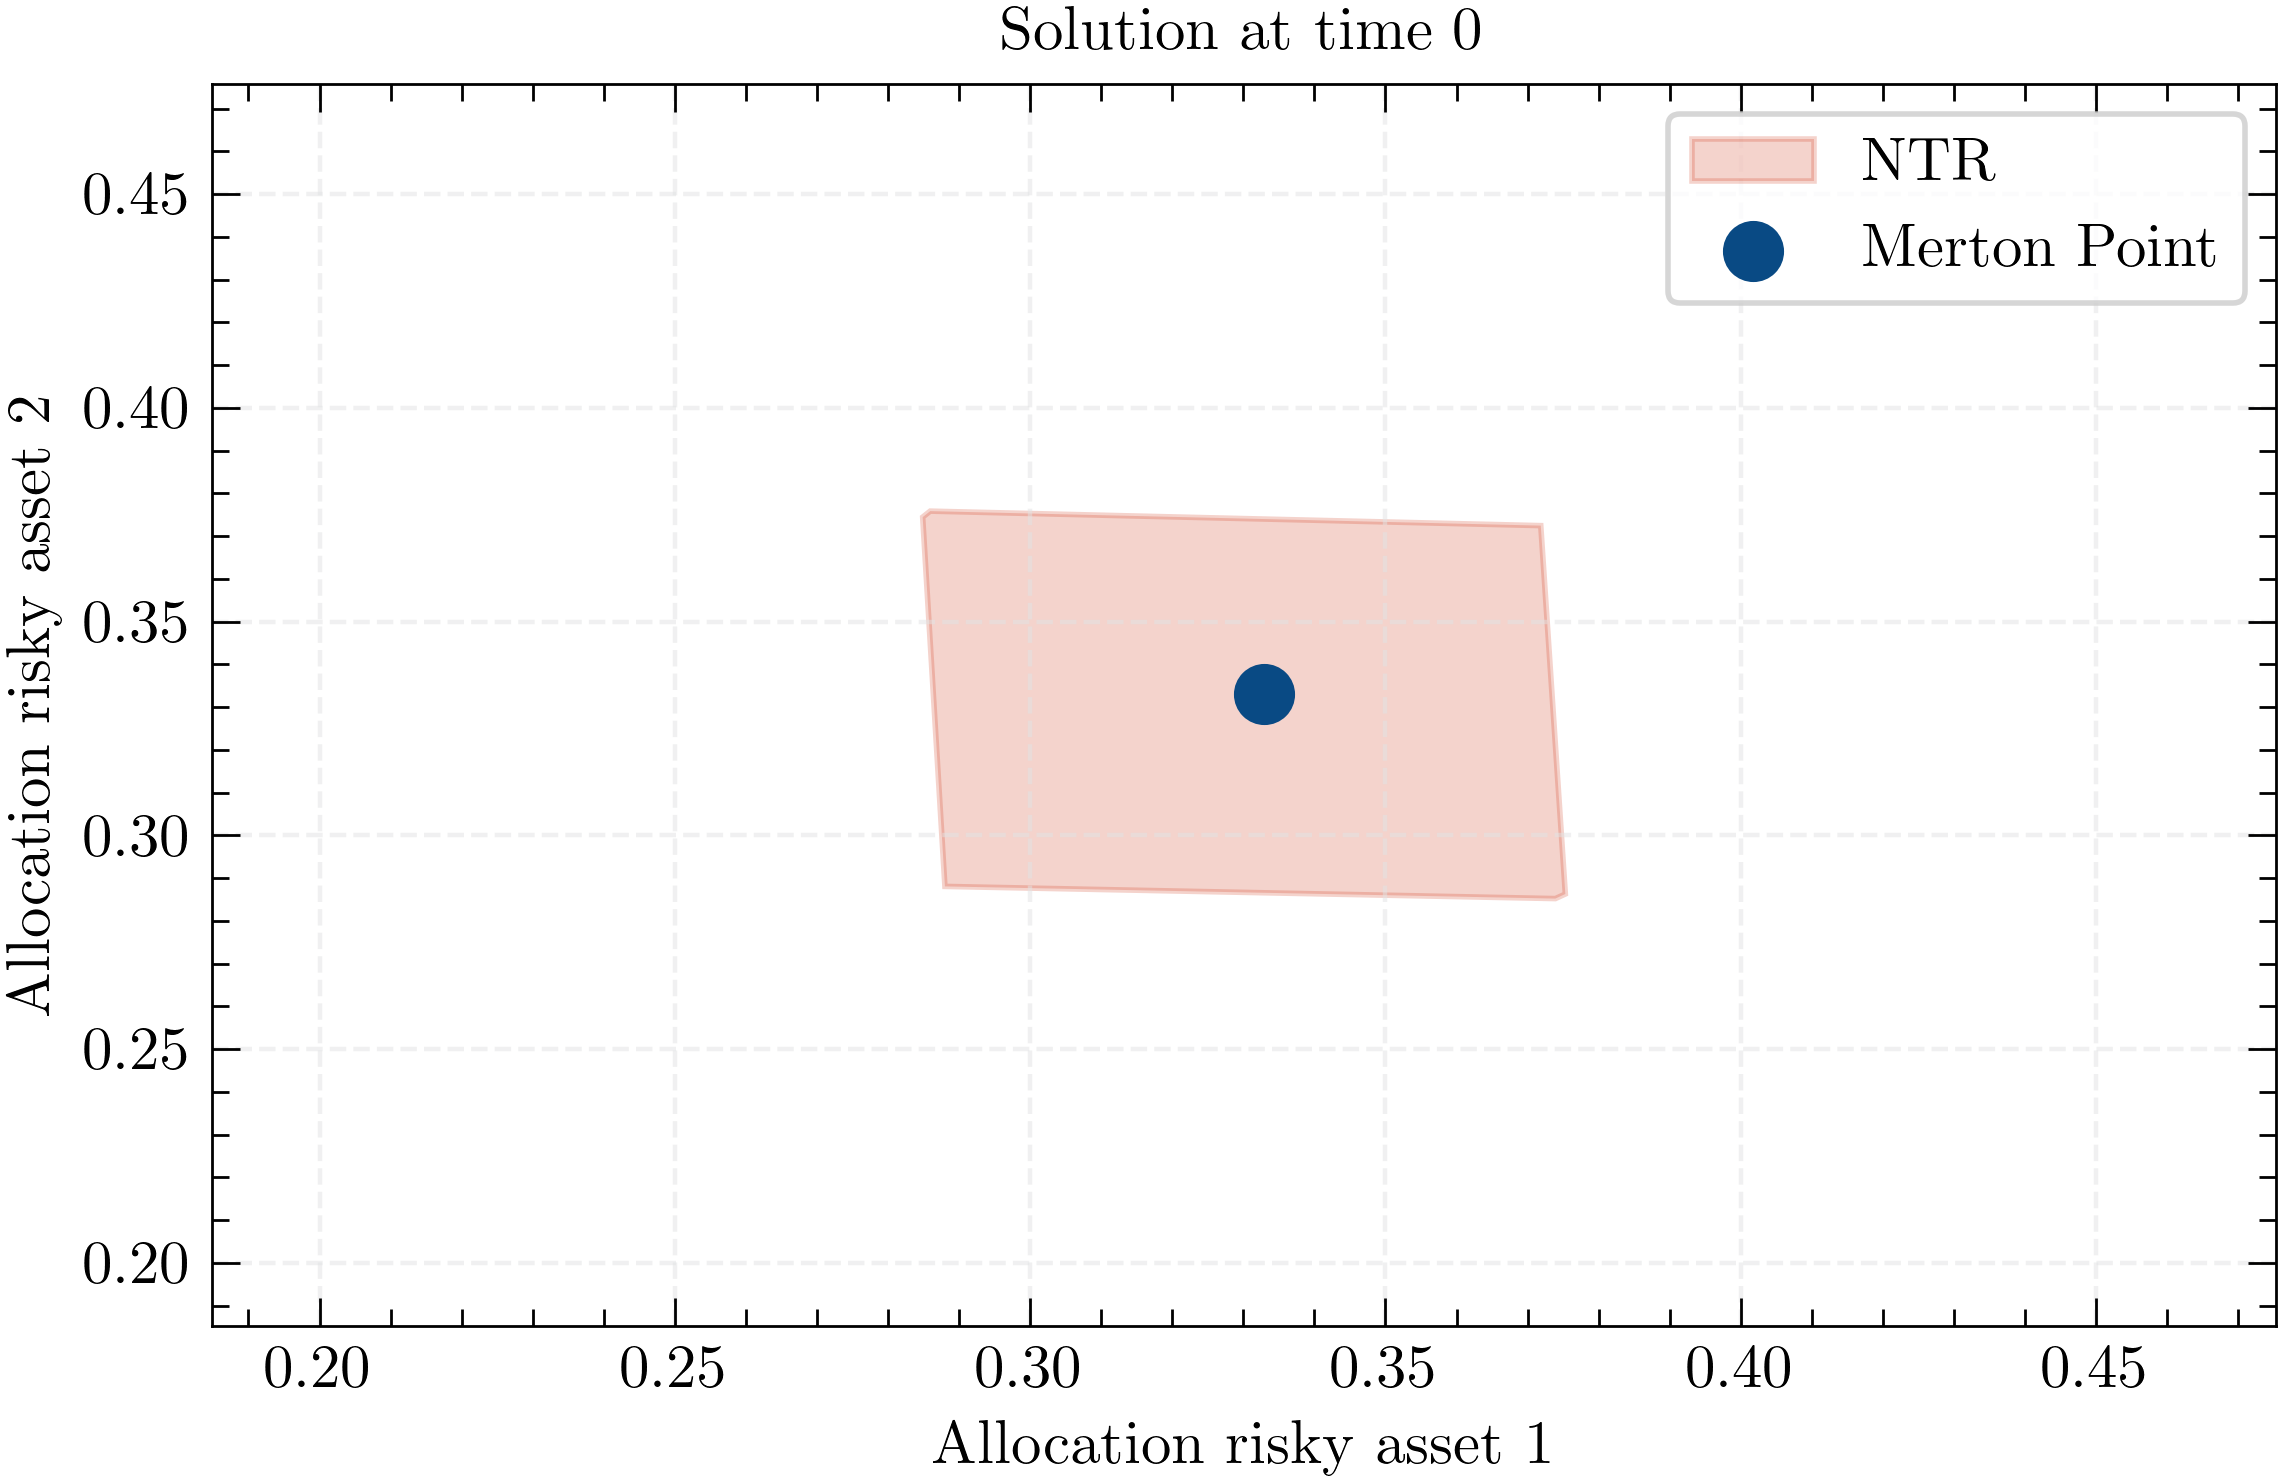
\includegraphics[scale=0.45]{NTR_Cai_Identical_d2_tau_0.005__no_consumption_t_0.png}
        \caption{No Trade Region for Independent Identically Distributed Assets.}
        \label{fig:NTR_2d_iid}
    \end{subfigure}

    % Space between the top and the bottom row
    \vspace{1em}

    % Bottom figures side by side
    \begin{subfigure}[t]{0.48\textwidth}
        \centering
        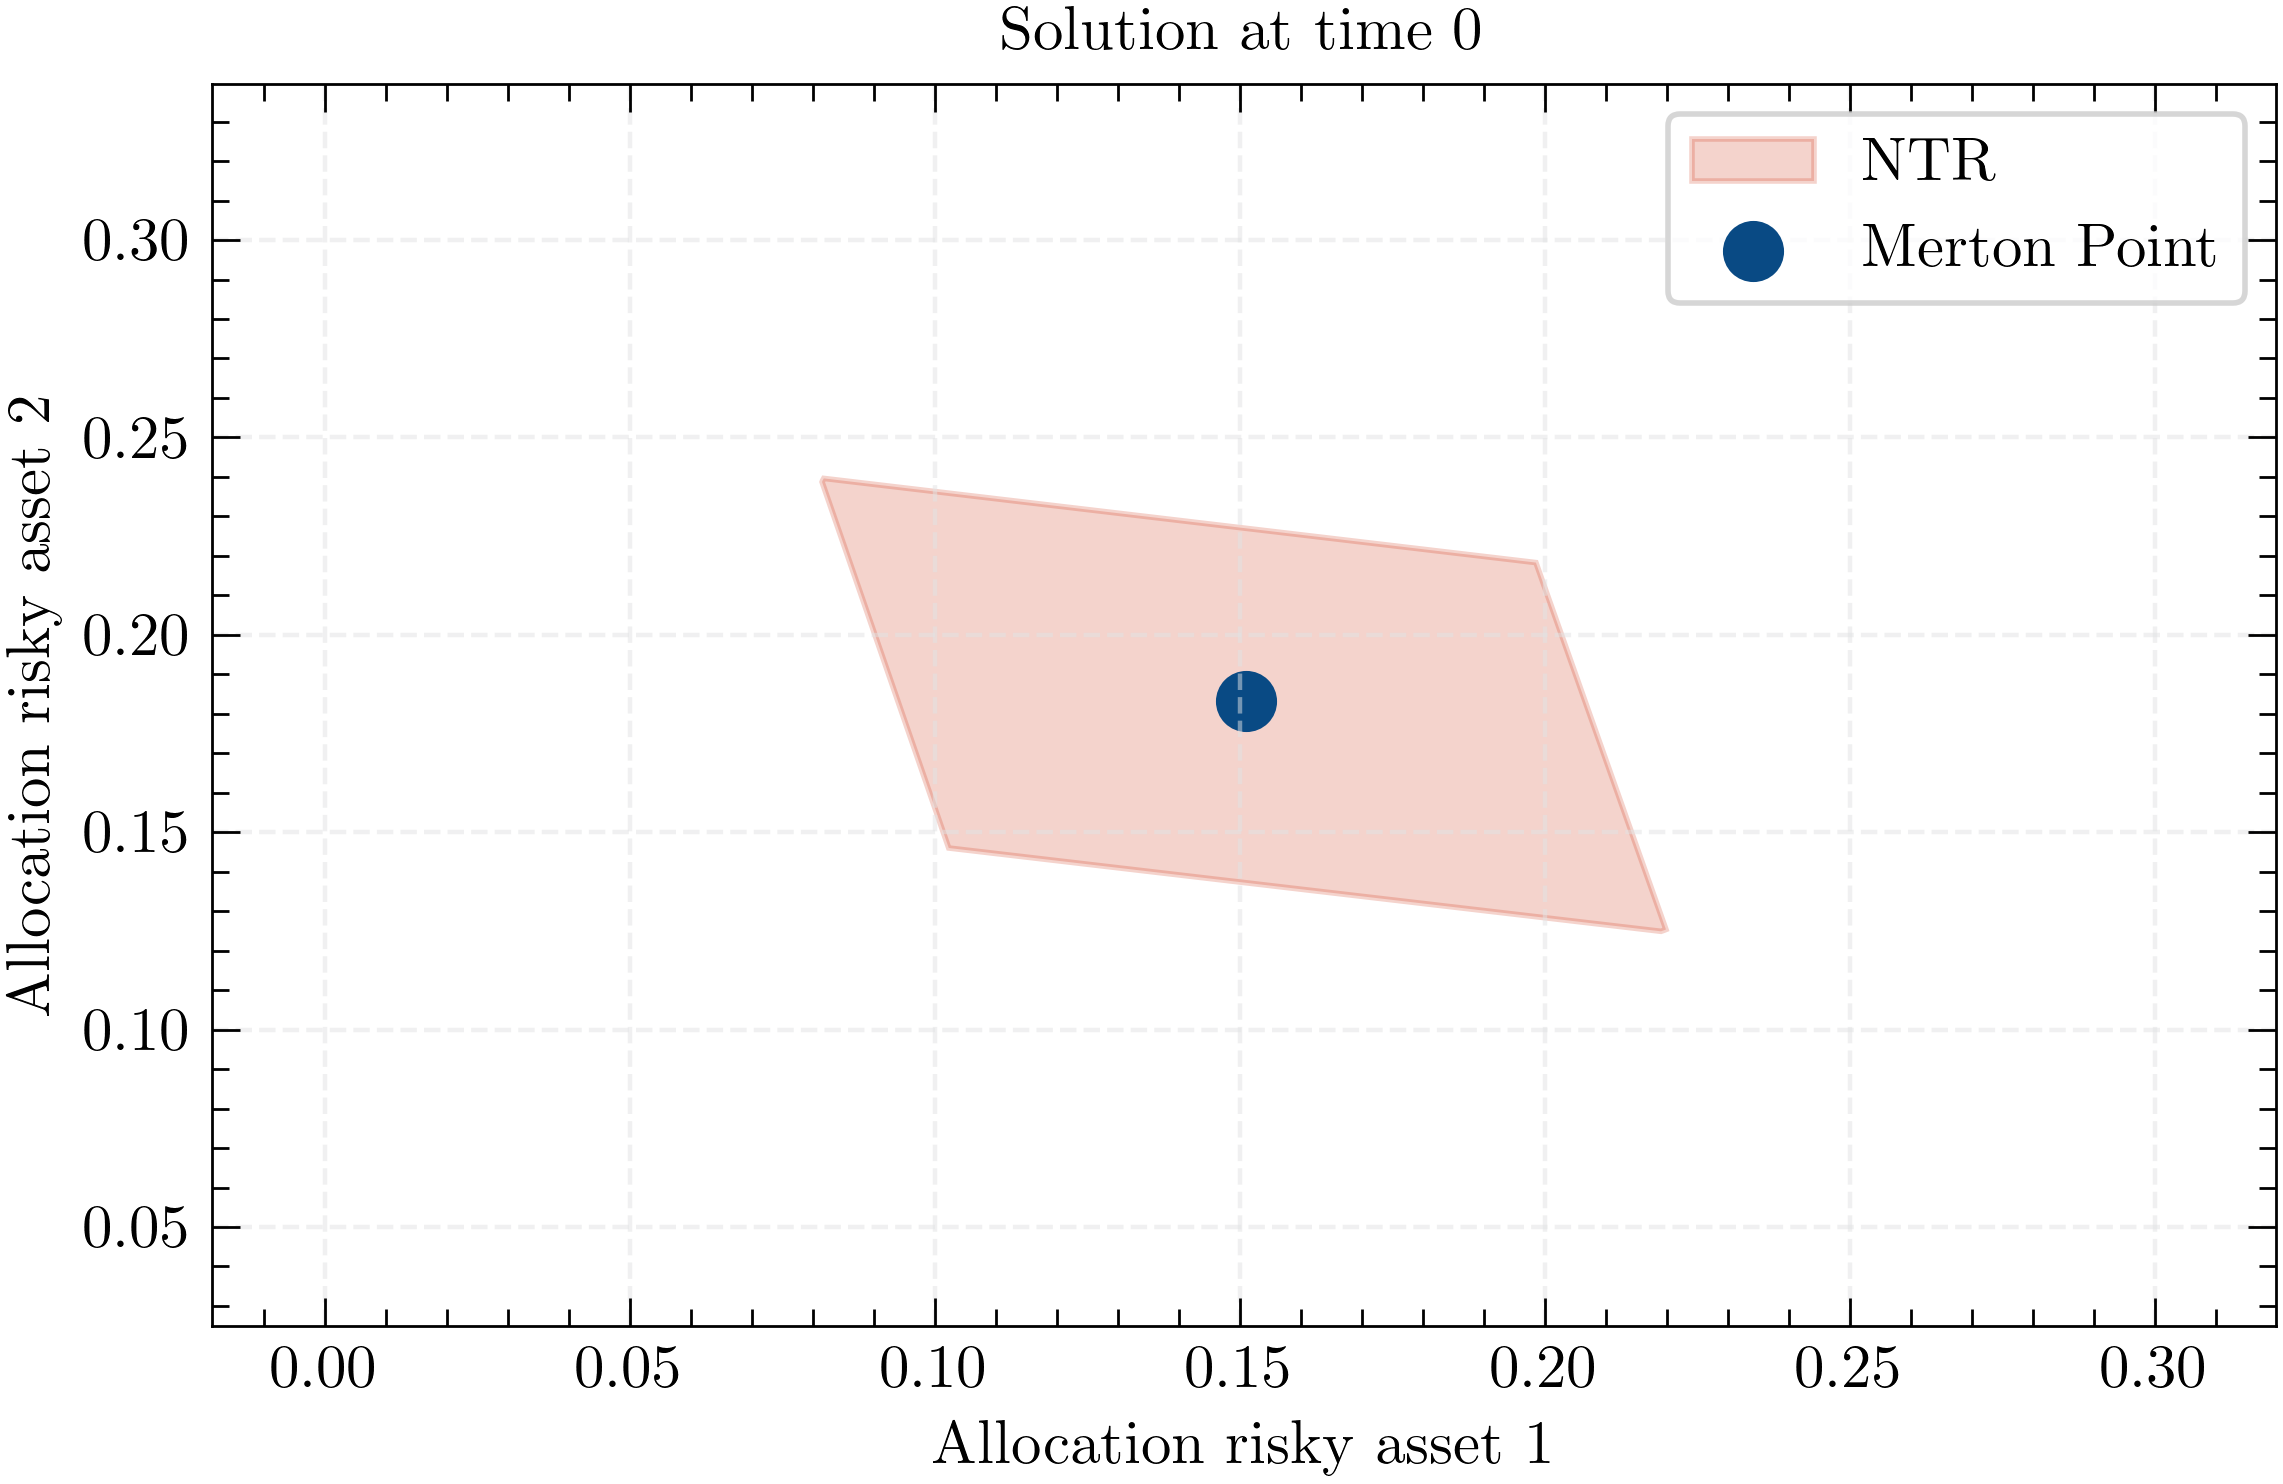
\includegraphics[scale=0.45]{NTR_Schober_Parameters_d2_tau_0.005__no_consumption_t_0.png}
        \caption{No Trade Region for Schober Parameters.}
        \label{fig:NTR_2d_Schober}
    \end{subfigure}%
    \hfill
    \begin{subfigure}[t]{0.48\textwidth}
        \centering
        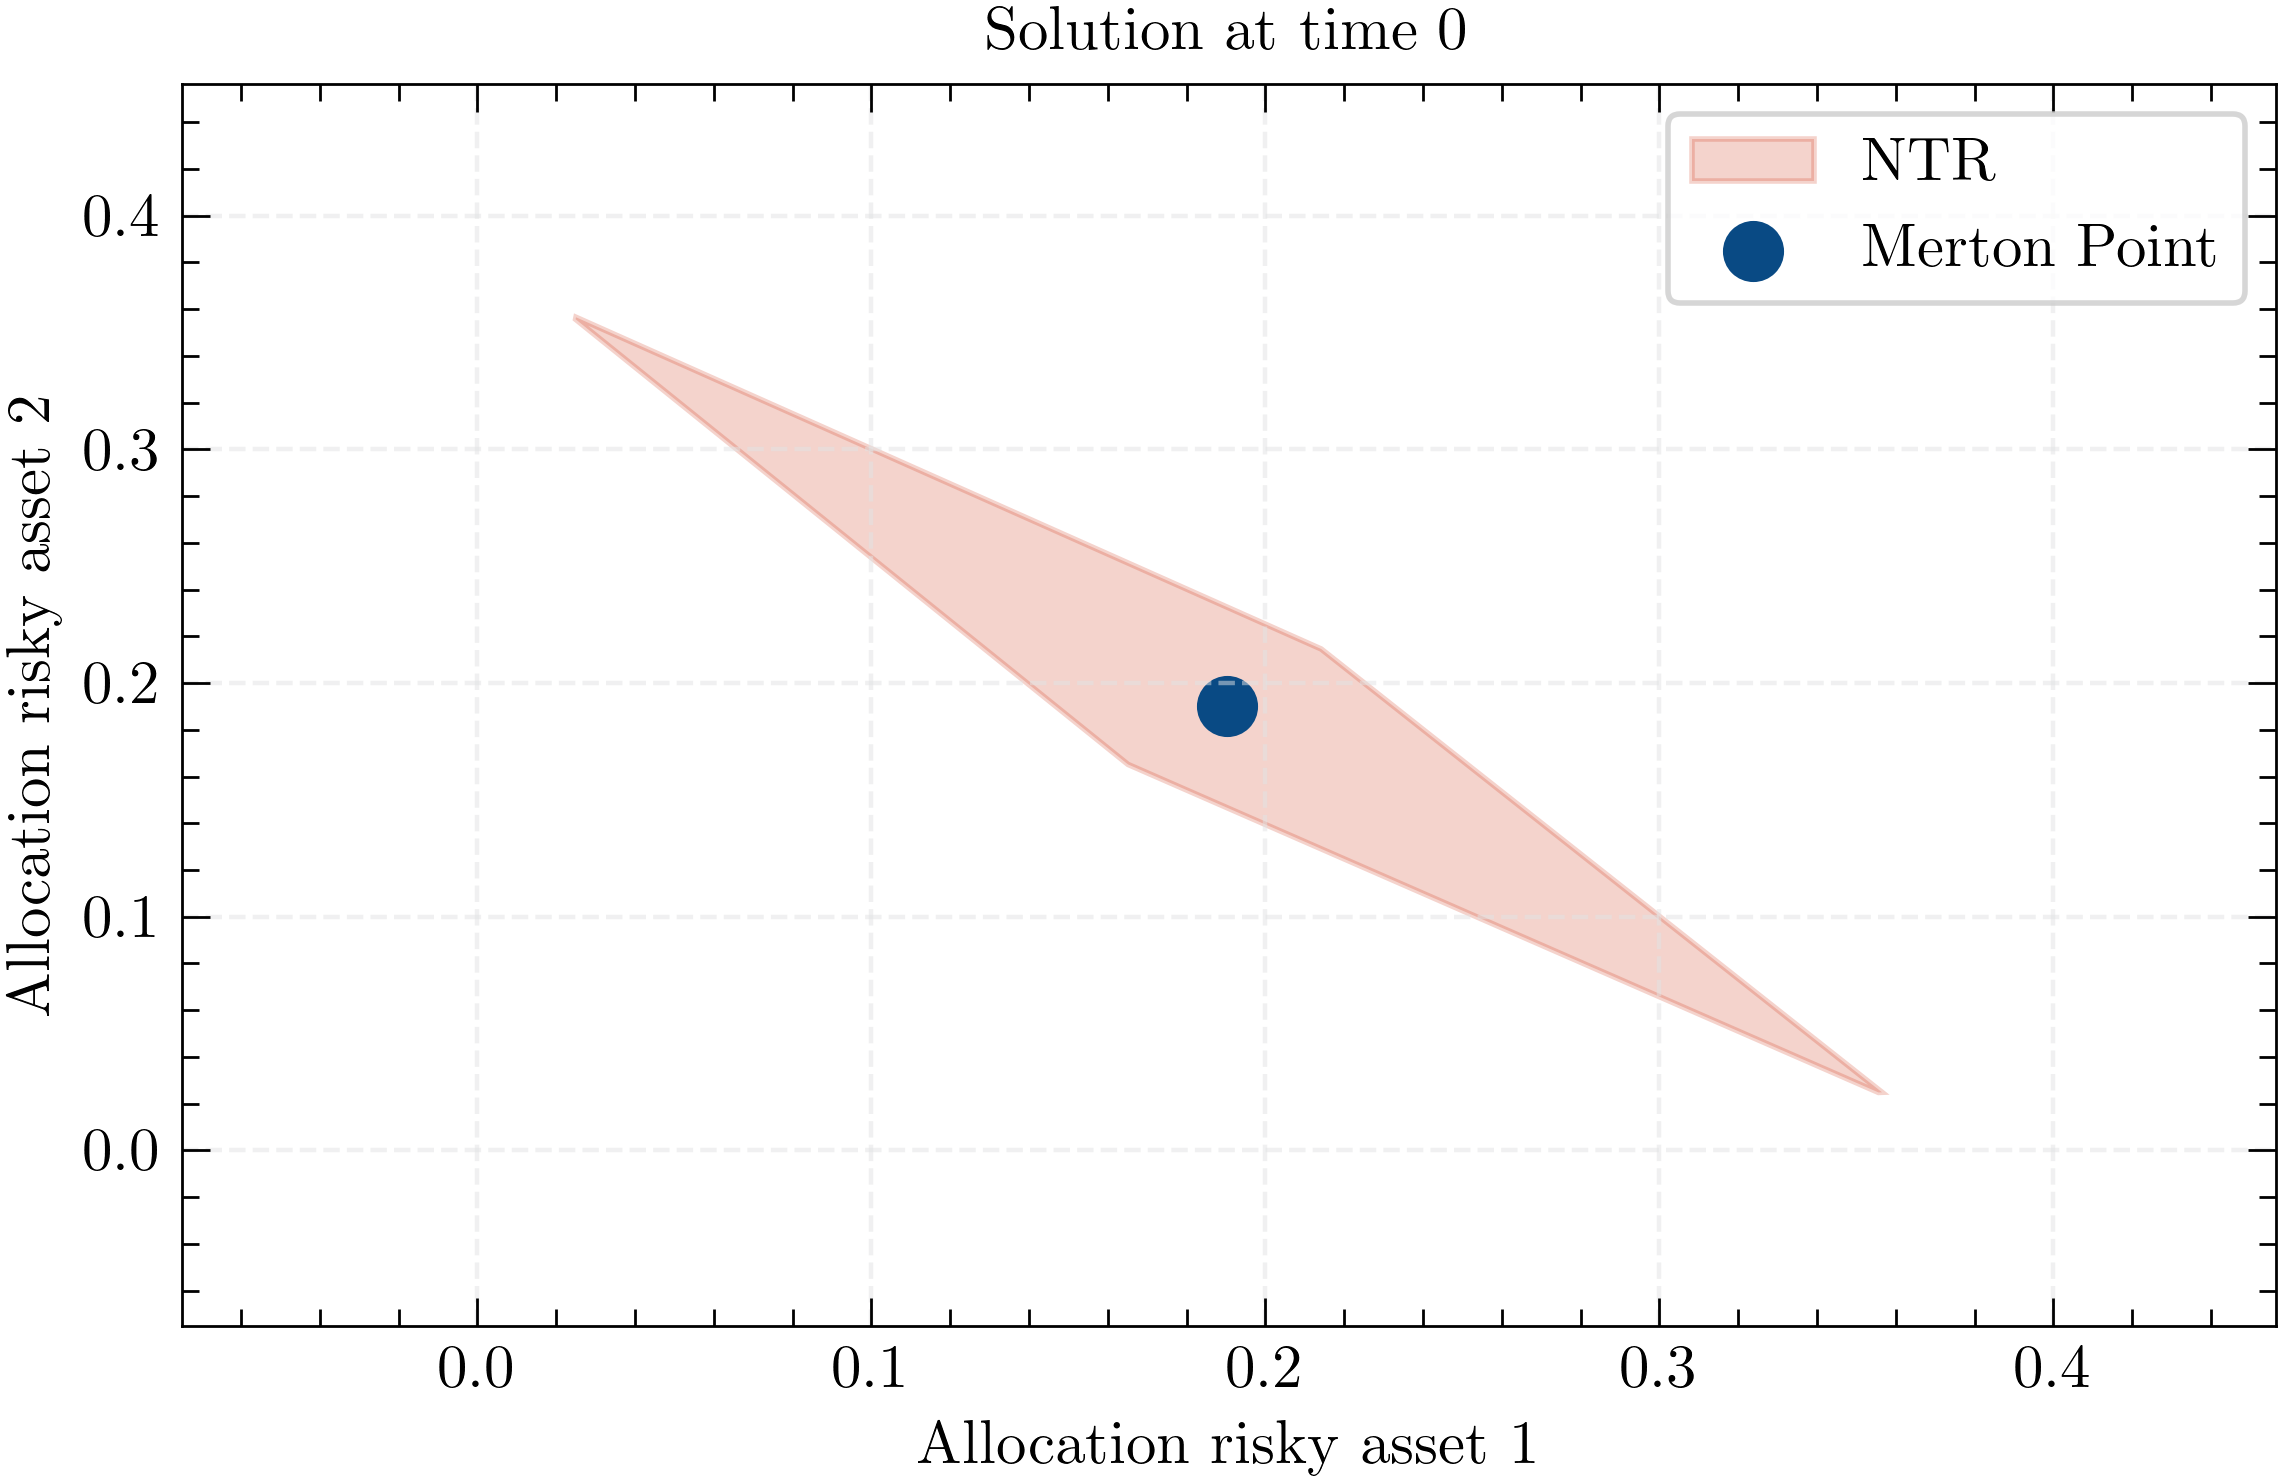
\includegraphics[scale=0.45]{NTR_Cai_High_Correlation_d2_tau_0.005__no_consumption_t_0.png}
        \caption{No Trade Region for High Correlation.}
        \label{fig:NTR_2d_High_Correlation}
    \end{subfigure}

    % Overall caption
    \caption{Comparison of No Trade Regions.}
    \label{fig:comparison_NTR}
\end{figure}
I note that for each of the parameterizations the No-Trade region is a rectangle or parallelogram.
For the case of identical and independent assets, the No-Trade region is a perfect square, whereas for the Schober parameters and the high correlation case,
the No-Trade region is a parallelogram. This is due to the correlation between the assets. When some correlation is present, the No-Trade region is skewed,
since some allocations which would be optimal in the absence of correlation are no longer optimal.

\subsubsection{Verifying the geometric shape of the No-trade Region}\label{Subsubsection: ConfirmShape}
Since much of the procedure for solving this problem, and approximating the NTR, leverages
the a-priori assumptions regarding the geometric shape of the NTR, i first want to verify that the
NTR indeed has $4$ vertices for the 2d case and is a convex hull.\\
In order to do this, i do a small modification to the solution algorithm proposed earlier.
Instead of computing vertices using $2^{d}$ predetermined points, i will instead
sample a larger set of points, ($2^7 = 128$) covering the boundaries of the feasible state space.
For each of these points i then solve the optimization problem,
and plot the solution, from allocations $\mathbf{x}_{t}$ and their solutions to the problem $\hat{\boldsymbol{\omega}}_{t}$.
I do this by using my original sample scheme, and adding mid-points between points,
which either sum to $1.0$ or have $0.0$ as allocation for one of the assets.
I consider the i.i.d case and the high correlation case, with $tau = 1\%$. I have increased the costs slightly in order to increase the
size of the NTR. This is to ensure that points also converge towards the faces and not only the verticies.
This is akin the the green regions in Figure \ref{fig:no_trade_region_schematic}.
Otherwise i would need more points. I plot the solutions for next to last period with investment decisions $T-2$.
The solutions are plotted below.

\begin{figure}[!ht]
    \centering
    \begin{subfigure}[t]{0.48\textwidth}
        \centering
        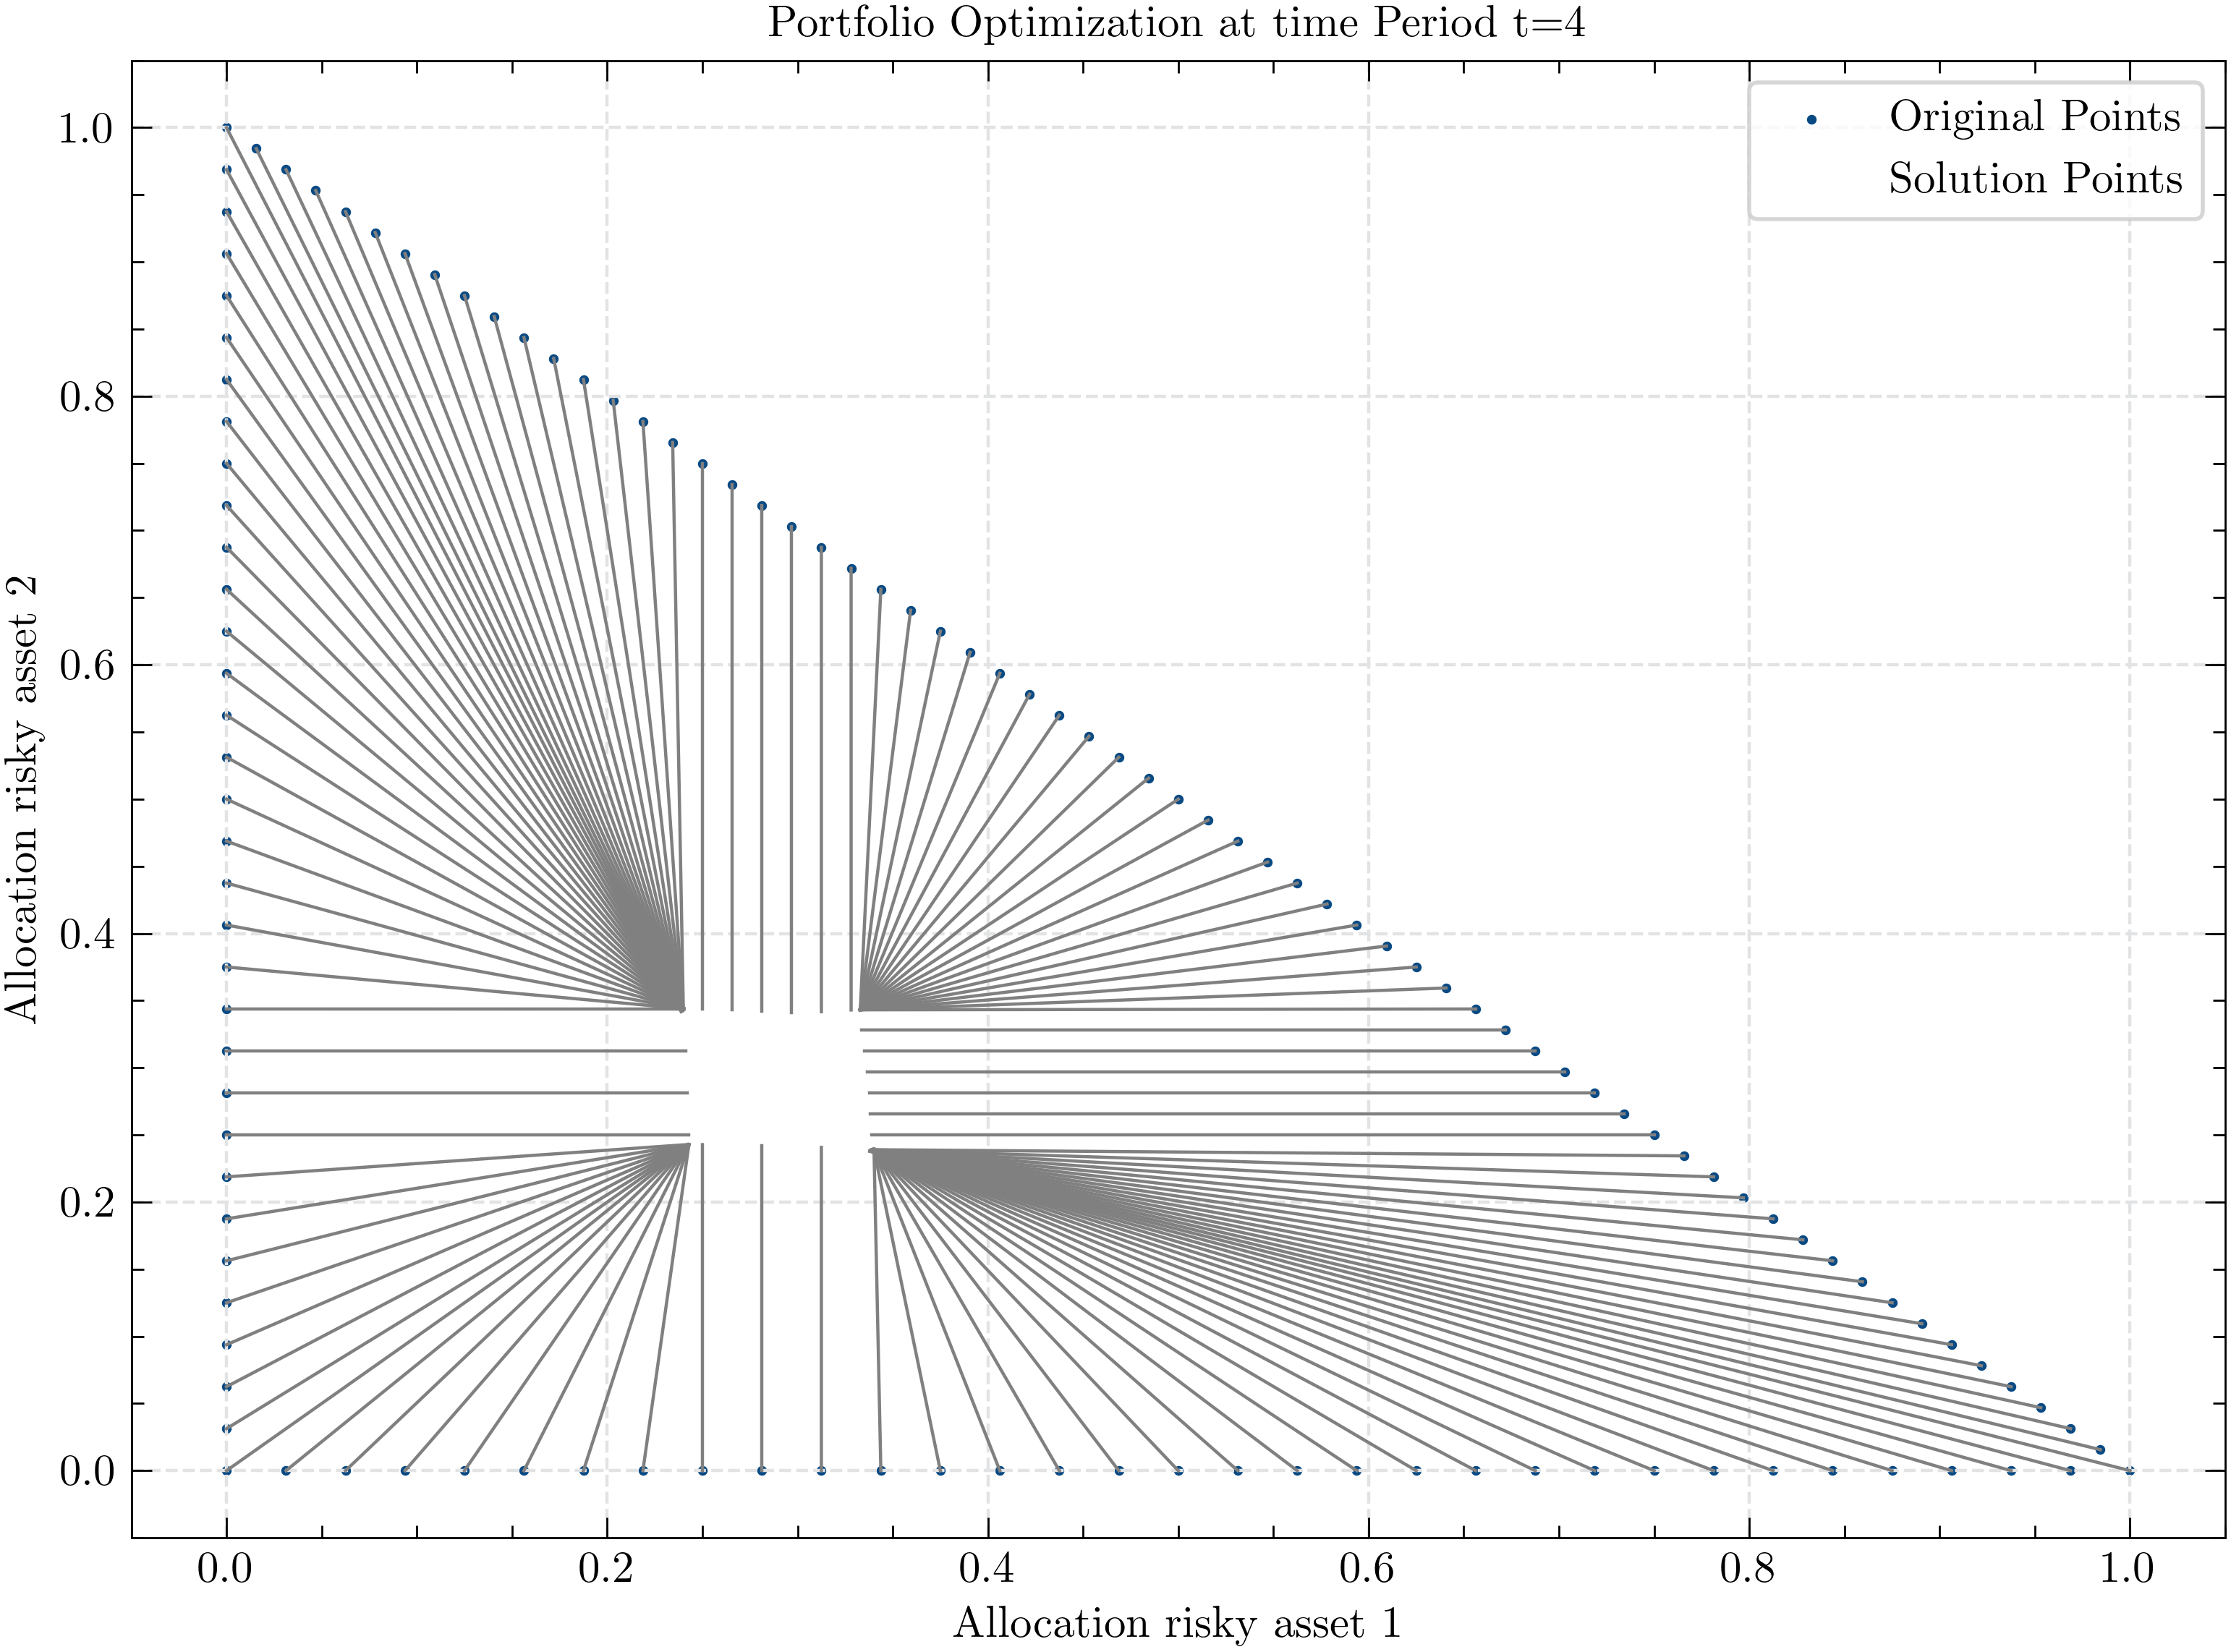
\includegraphics[scale = 0.36]{Verify_NTRCai_Identical_t_4.png}
        \caption{Solutions to the i.i.d case with 2 assets in period $T-2$.}
        \label{fig:NTR_verify_iid}
    \end{subfigure}%
    \hfill
    \begin{subfigure}[t]{0.48\textwidth}
        \centering
        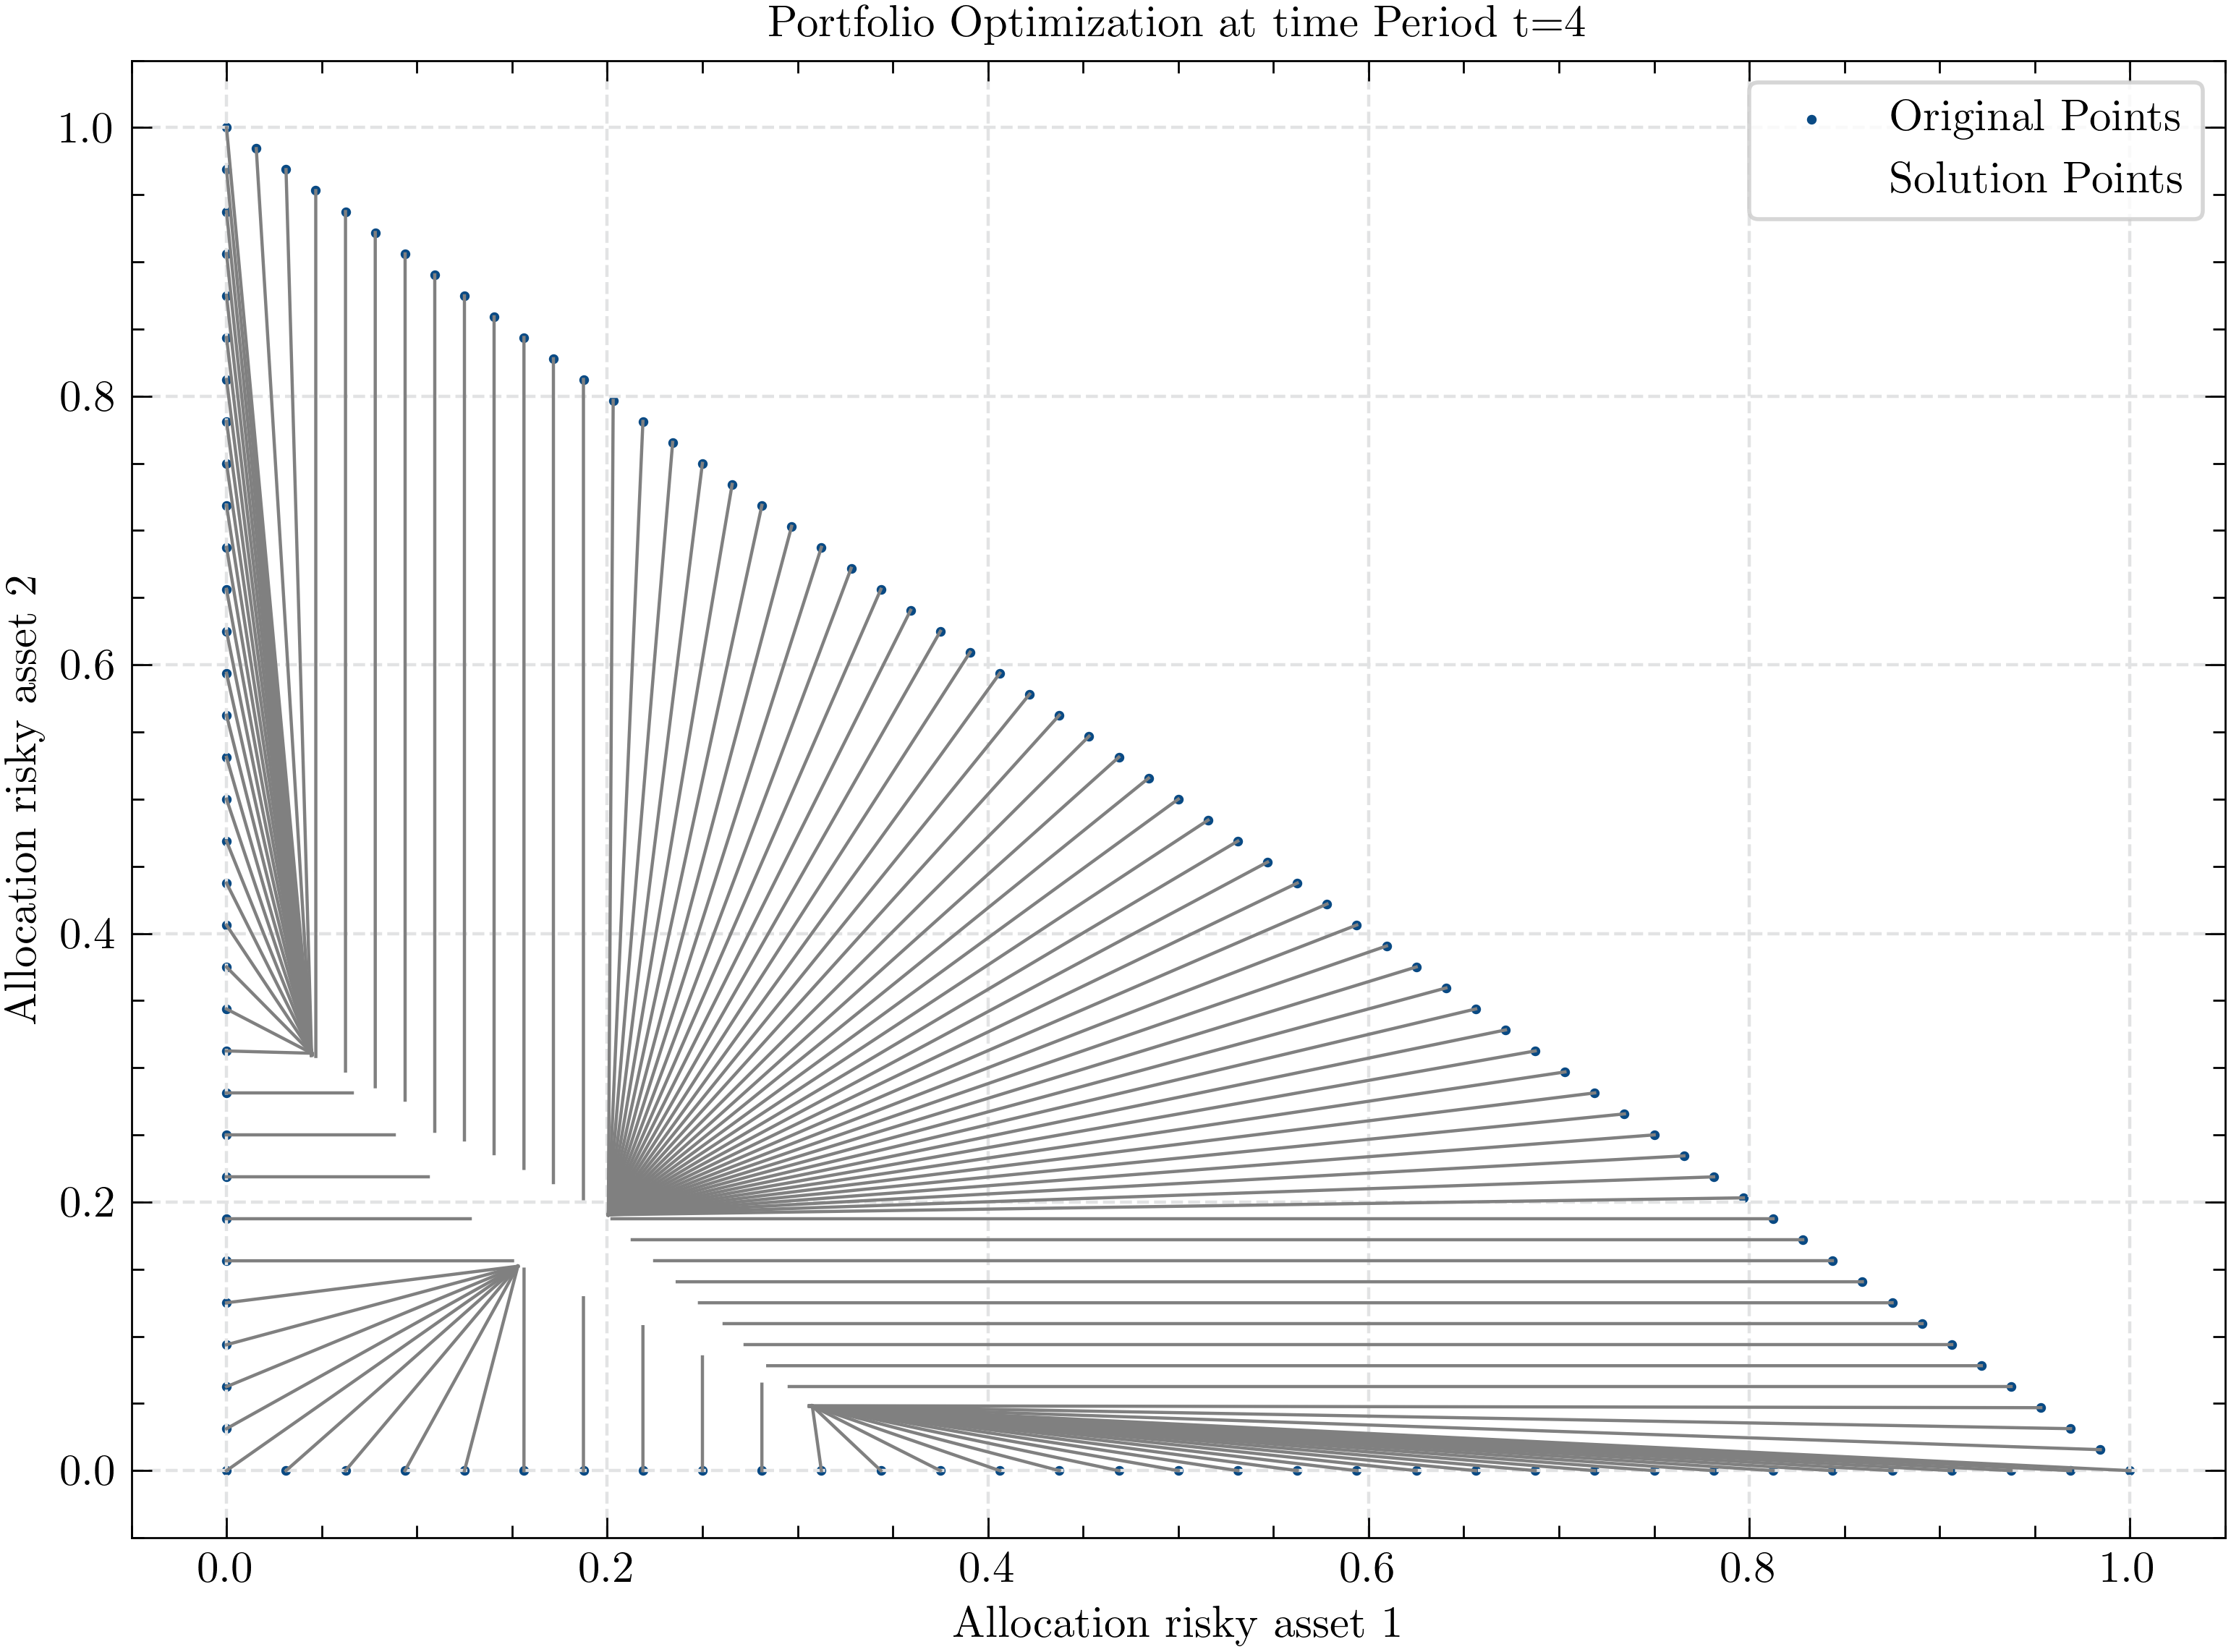
\includegraphics[scale = 0.36]{Verify_NTRCai_High_Correlation_t_4.png}
        \caption{Solutions to the high correlation case with 2 assets in period $T-2$.}
        \label{fig:NTR_verify_Correlation}
    \end{subfigure}

    % Overall caption
    \caption{Verifying the assumptions of the NTR iin $2$ dimensions.}
    \label{fig:NTR_Verify}
\end{figure}
I find that the assumptions regarding the \ac{NTR} are indeed correct in the two dimensional examples i have constructed.
Furthermore this verifies that the assumptions also hold for correlated asset, which was only postulated by \autocite{liu2002}.
Furthermore these plots also nicely confirm that the optimization process as a whole works as intended.
Further verification in higher dimensions are not considered. First of all \autocite{liu2002} confirms this formally in larger dimensions,
for the case of uncorrelated assets, and the intuition regarding the \ac{NTR} does not change when dimensionality is increased.

\subsubsection{Investigating the No-Trade Region} \label{Subsubsection: InvestigatingNTR}
We now look at the No-Trade region for the base model with proportional transaction costs and no consumption in more detail.
Specifically we look at how the region behaves over the entire investment horizon $[0, T]$, and how the region changes with different transaction cost levels.
We choose to look at the model with the Schober parameters, as this is a mixture of the other two parameterizations.

\begin{figure}[!ht]
    \centering
    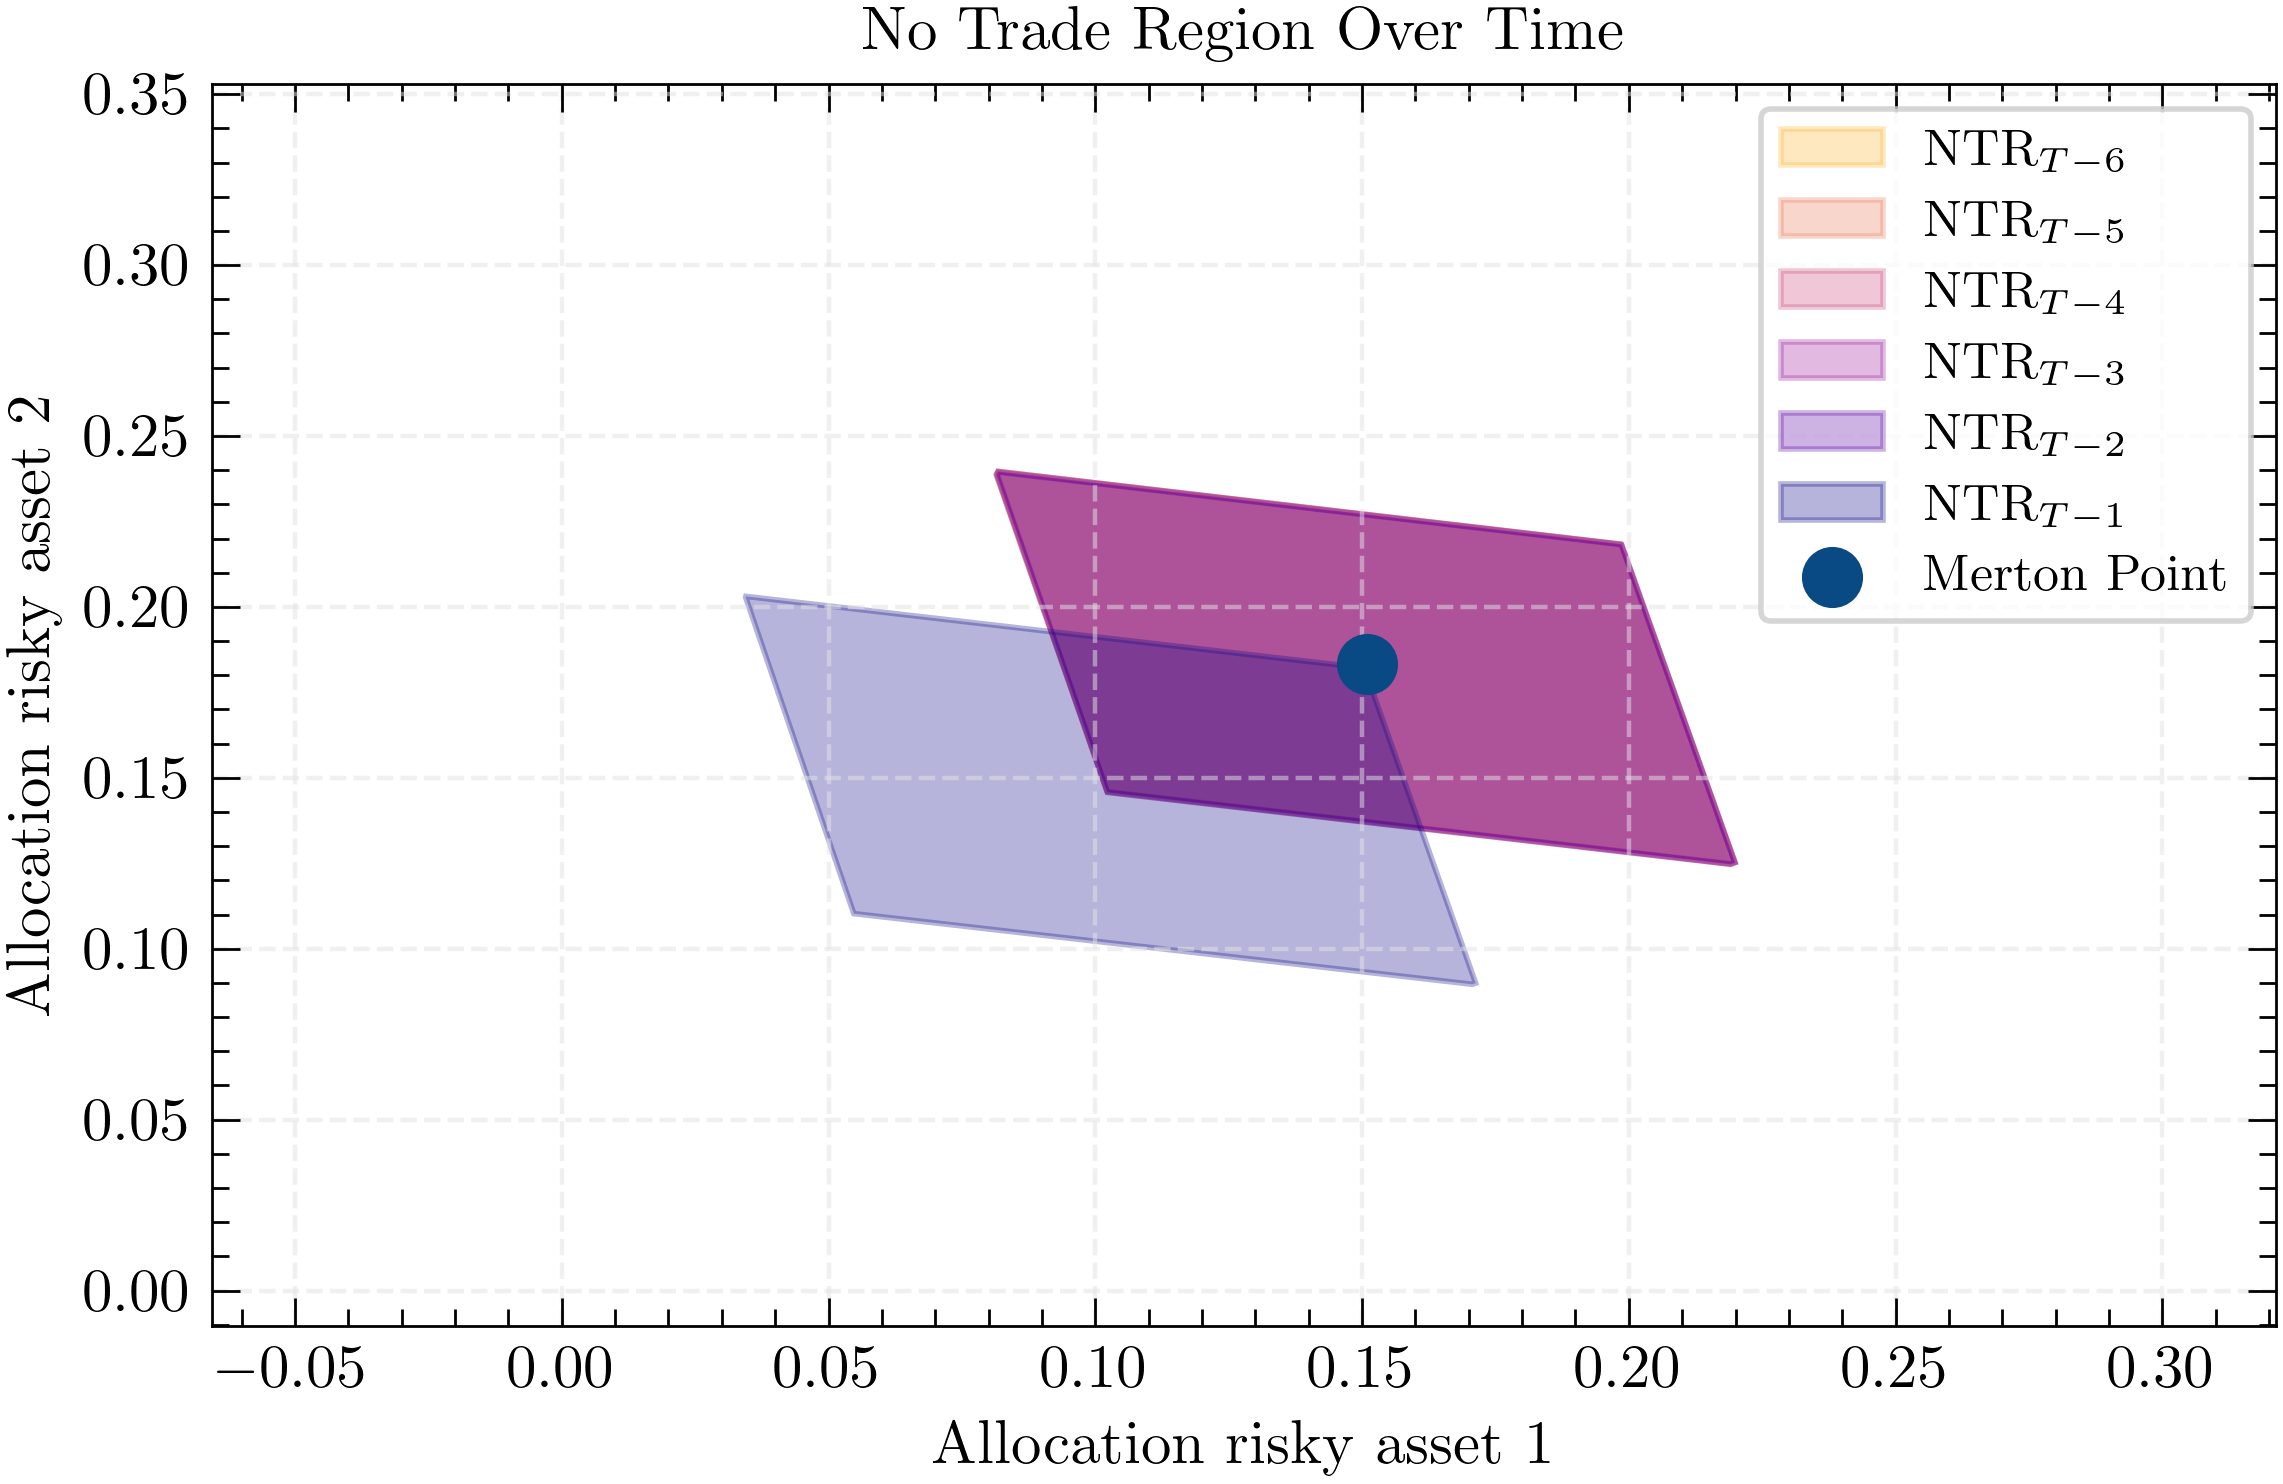
\includegraphics[scale = 0.45]{NTR_Schober_Parameters_d2_tau_0.005__no_consumption_Over_Time_t_5.png}
    \caption{No Trade Region for Schober Parameters over Time.}
    \label{fig:NTR_2d_iid_standalone}
    \floatfoot{The No-Trade region is plotted for the Schober parameters over the entire investment horizon $[0, T-1]$
    For time points $t\in [0,T-2]$ the \ac{NTR}s overlap.}
\end{figure}

I note that at the last time point $t = T-1$ the \ac{NTR} moves away from the merton point towards the origin, and the Merton point is is
now the upper right corner of the \ac{NTR}. For all other time periods the \ac{NTR} is the same, and the Merton point is in the center.

\begin{figure}[!ht]
    \centering
    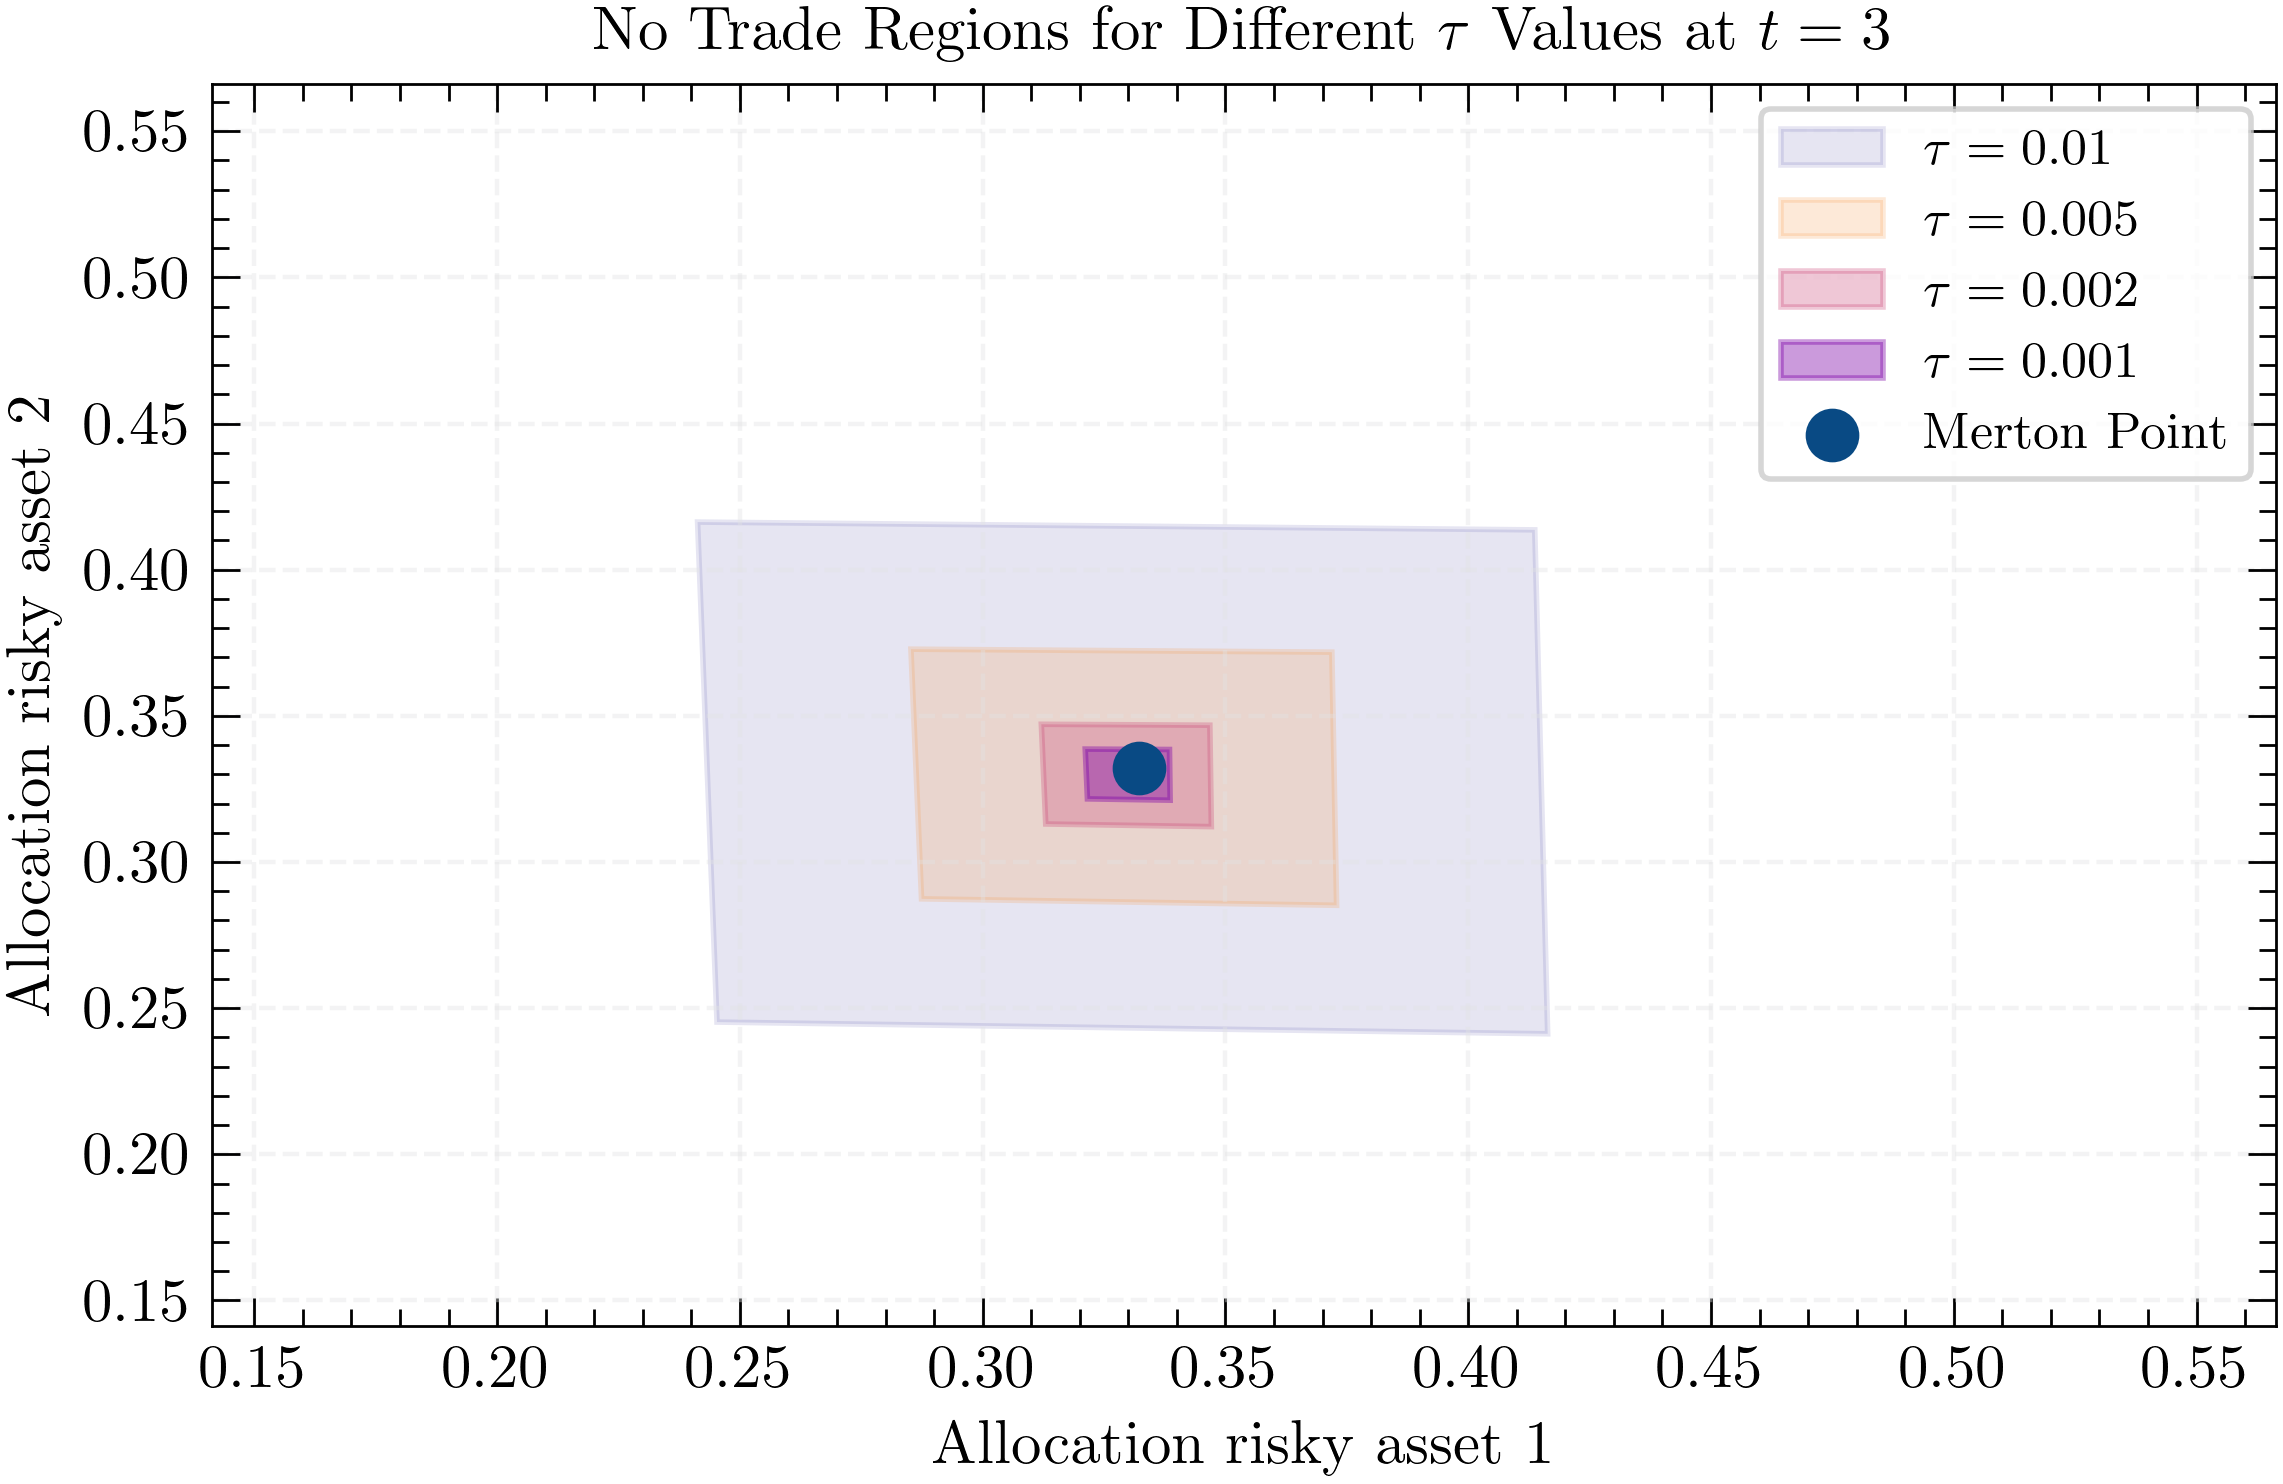
\includegraphics[scale = 0.45]{NTR_Cai_IdenticalDifferent_Tau_t_3.png}
    \caption{No Trade Region for the iid Parameters with different values of $\tau$.}
    \label{fig:NTR_2d_iid_tau_analysis}
\end{figure}
I now investigate how the No-Trade region changes with different transaction cost levels.
I do this for the i.i.d. parameters, and plot the \ac{NTR} for different values of $\tau$ in \autoref{fig:NTR_2d_iid_tau_analysis}.
When the transaction costs are increased, the \ac{NTR} increases aswell and vice-versa. 
I note that for low enough transaction costs, the \ac{NTR} shrinks towards the Merton point.
However when transaction costs are low enough, the Merton point is not in the excact center, which might signify that at low enough values, some numerical instabilities from the
minimizer, and function approximation using \ac{GPR} might be present.

\subsubsection{Increasing the dimensionality of the model} \label{Subsubsection: IncreasingDimensionality}
We now increase the dimensionality of the model to $d = 3$ and look at the No-Trade region for the Schober parameters and for the i.i.d parameters.

\begin{figure}[!ht]
    \centering
    \begin{subfigure}[t]{0.48\textwidth}
        \centering
        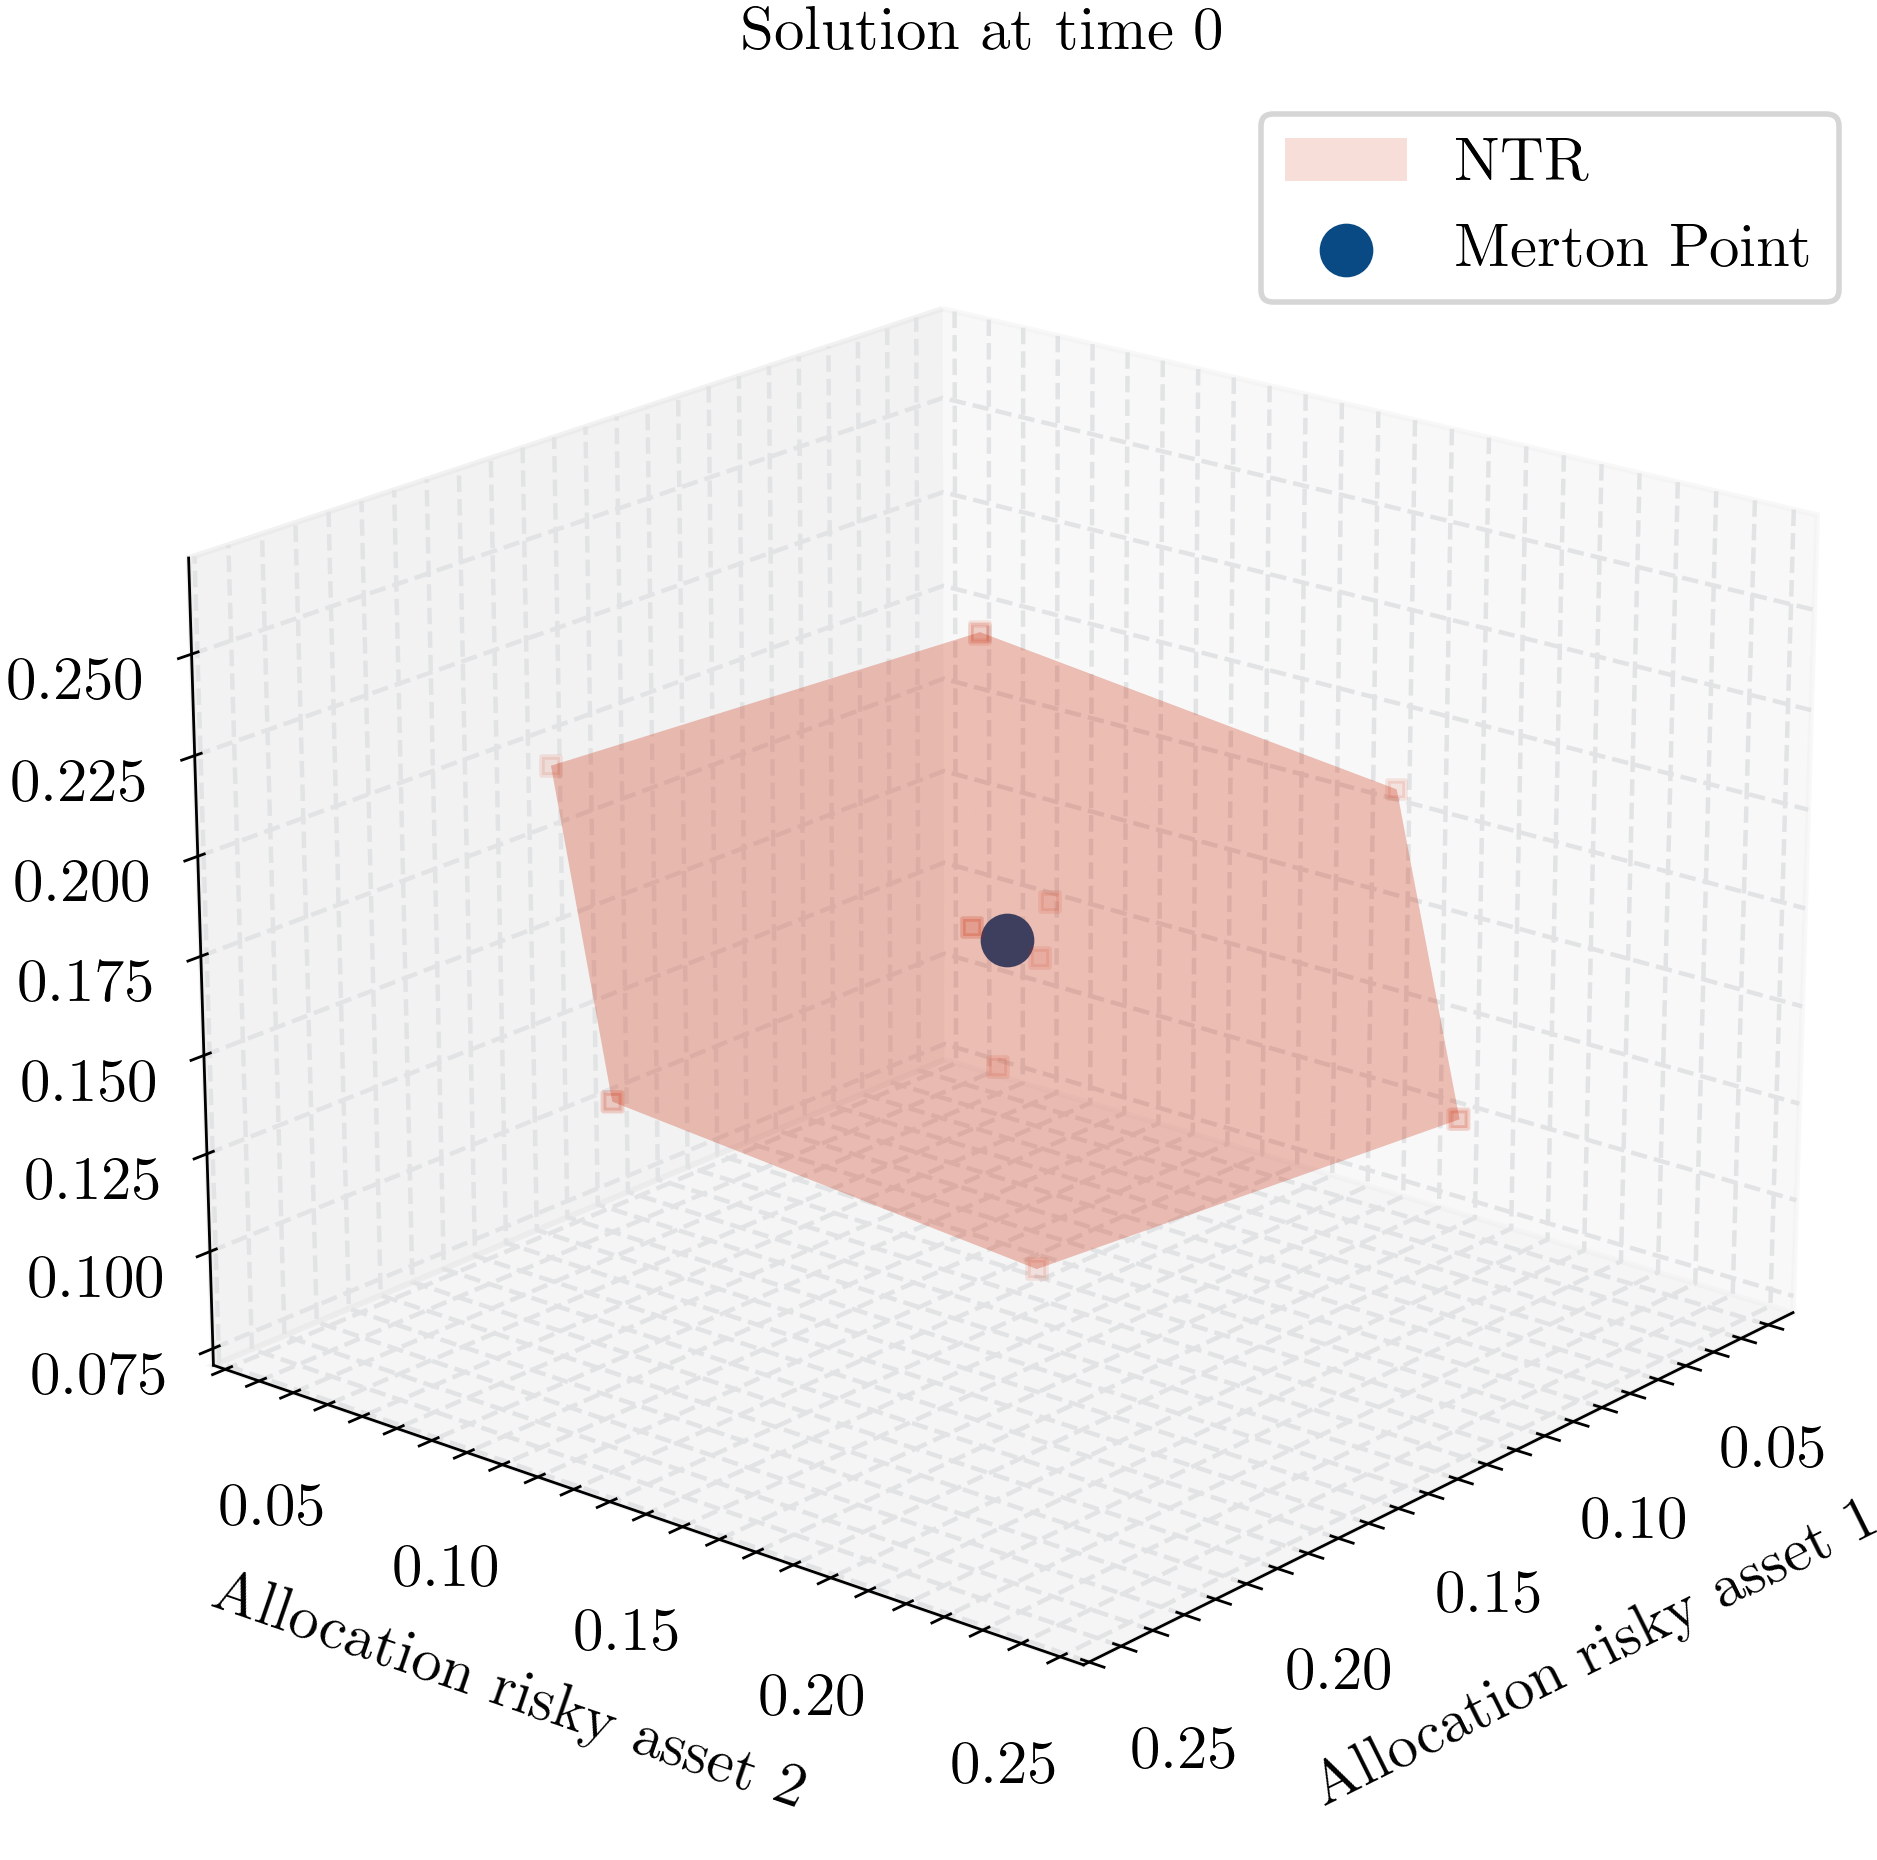
\includegraphics[scale = 0.45]{NTR_Schober_Parameters_d3_tau_0.005__no_consumption_t_0.png}
        \caption{No Trade Region for Schober Parameters in 3 dimensions.}
        \label{fig:NTR_3d_Schober}
    \end{subfigure}%
    \hfill
    \begin{subfigure}[t]{0.48\textwidth}
        \centering
        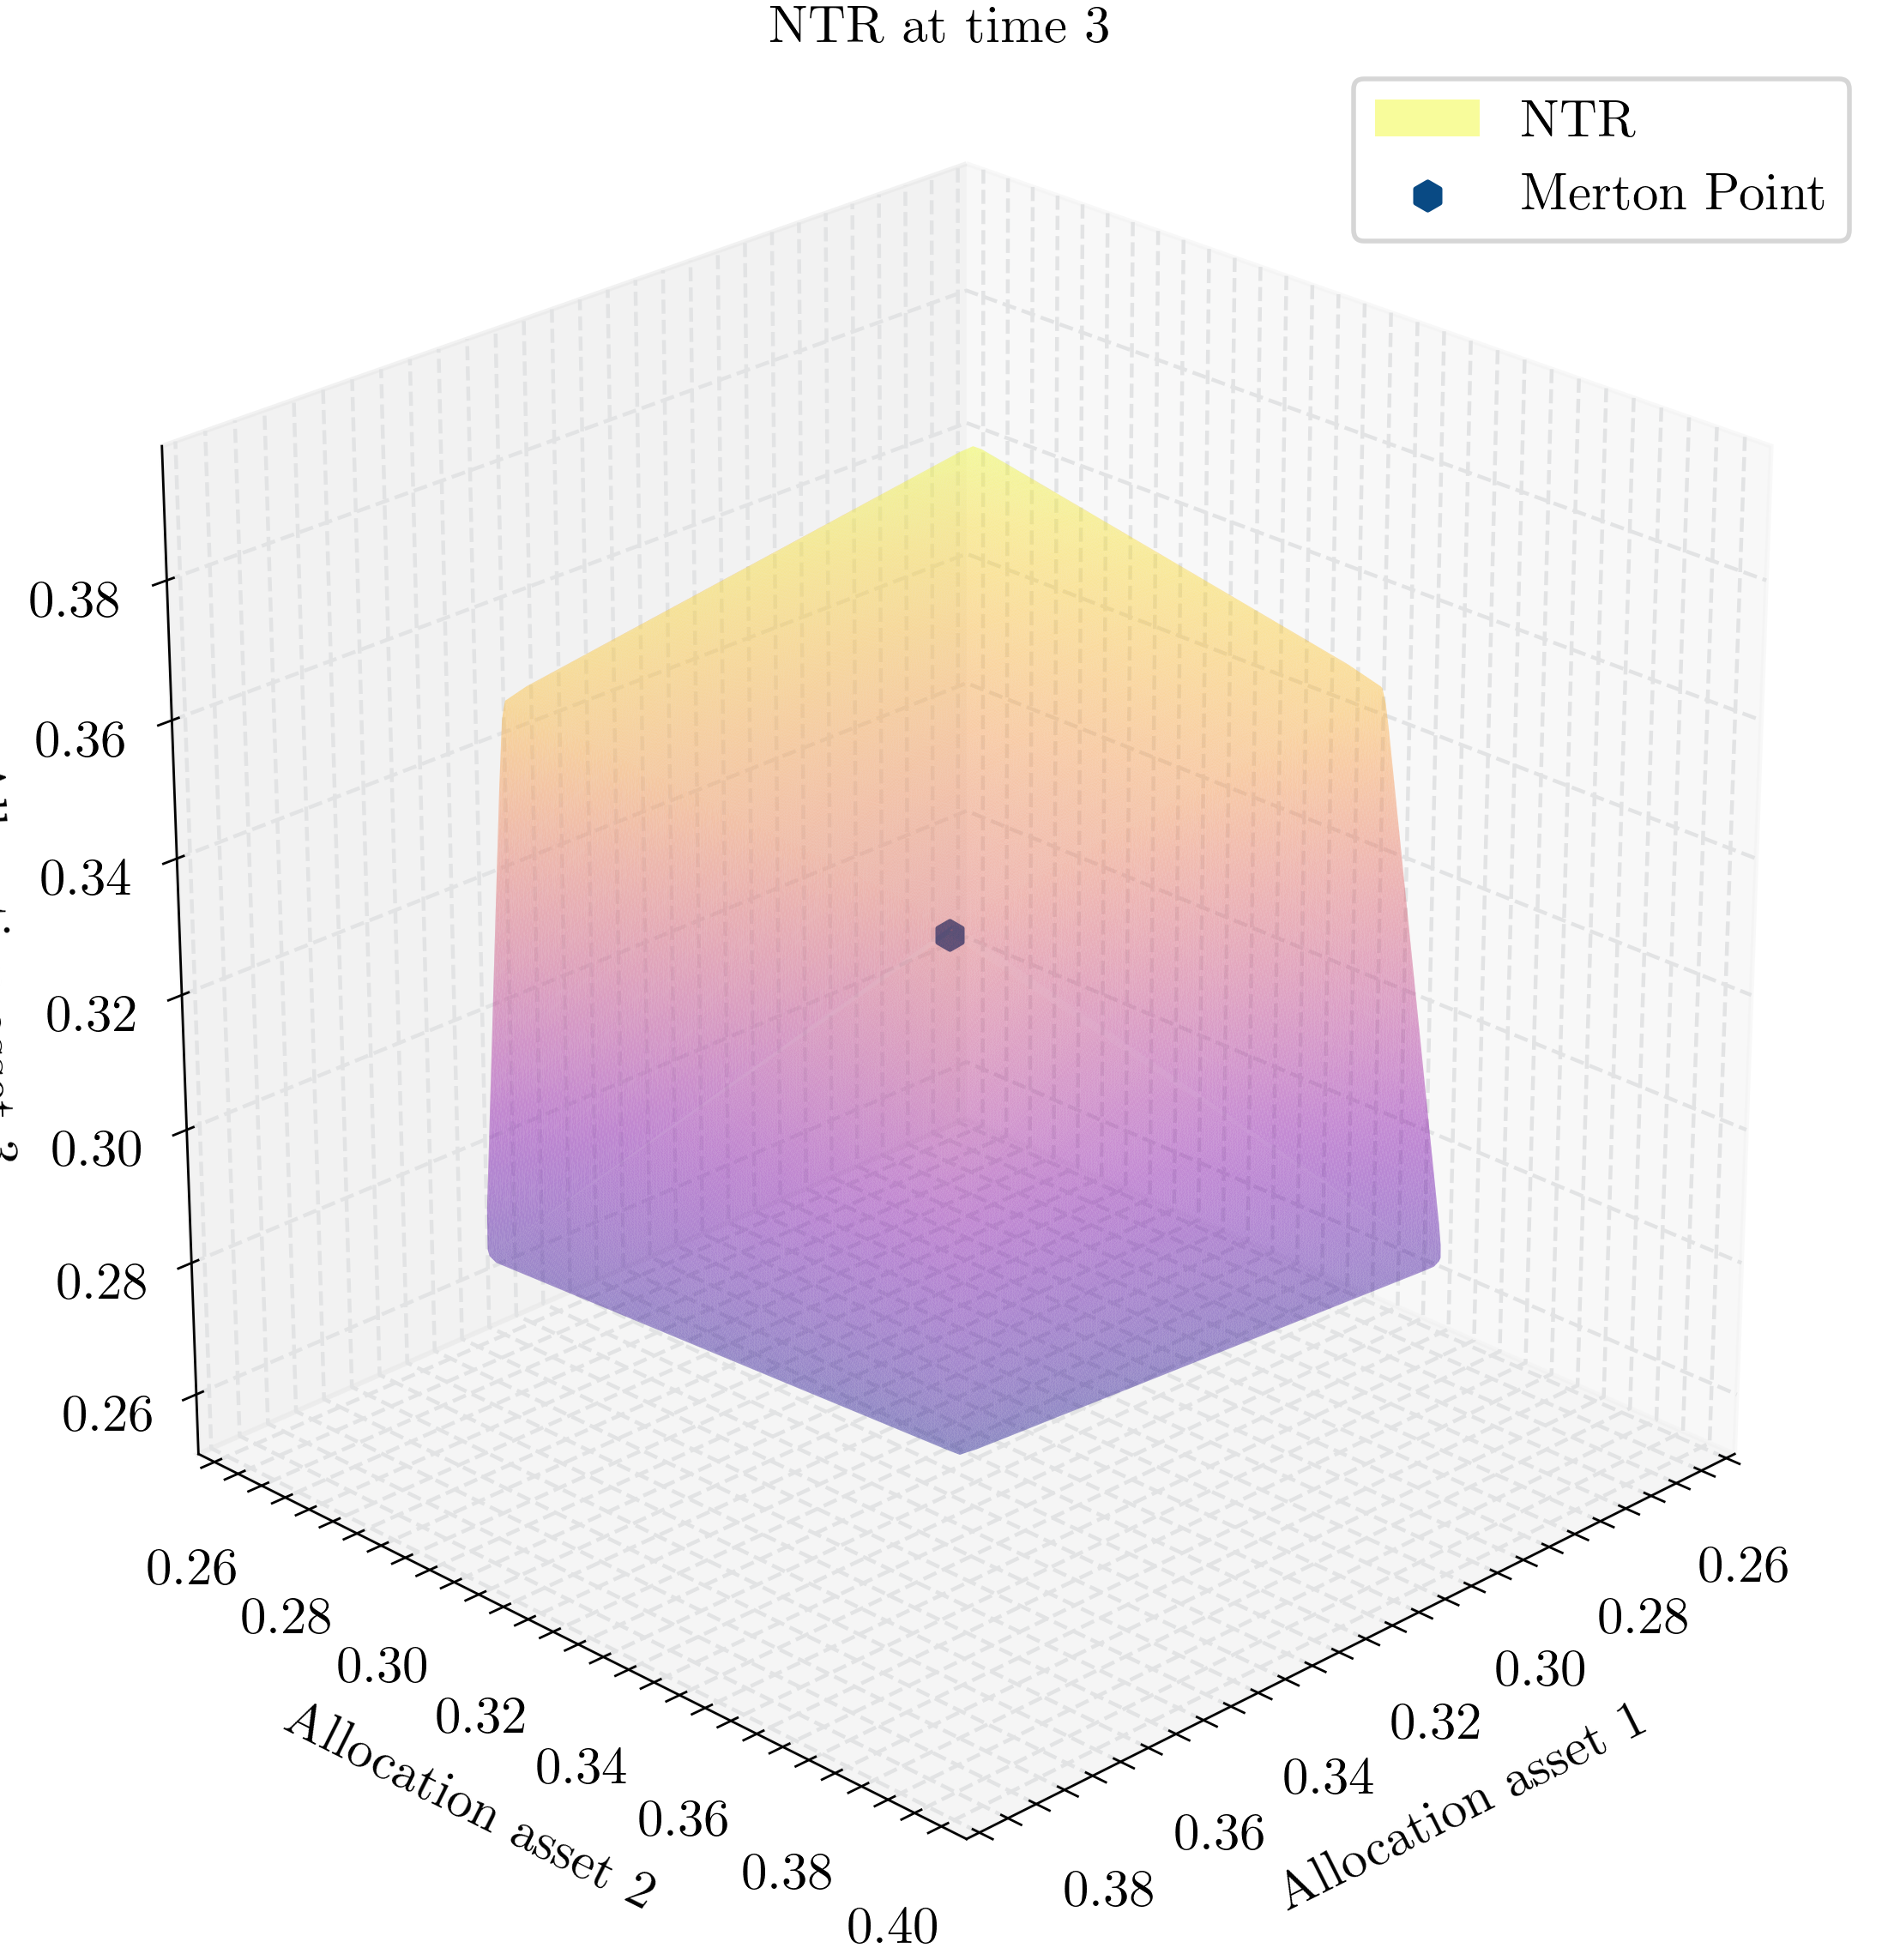
\includegraphics[scale = 0.45]{NTR_Cai_Identical_d3_tau_0.005__no_consumption_t_3.png}
        \caption{No Trade Region for i.i.d. Parameters in 3 dimensions}
        \label{fig:NTR_3d_iid_Correlation}
    \end{subfigure}

    % Overall caption
    \caption{Comparison of No Trade Regions.}
    \label{fig:comparison_NTR_3d}
\end{figure}
Note that the i.i.d NTR looks like a skewed cube, whereas this was a perfect square in the 2 dimensional case.
Looking that the points forming the convex hull that is the NTR, it is clear that the NTR is restricted by the no-borrowing constraint,
since one of the border points, which would otherwise form the perfect cube, would outside the feasible space if this was possible, and is then projected into the feasible space. 
Hence when the risky returns outweigh the risk-free return,
to such a degree that the merton point moves towards the boundary of the feasible space, cube like shapes are no longer possible.
In the $2$ dimension case, this is akin to the \ac{NTR} being close to the budget line, and the \ac{NTR} would then form a triangle.

This is clear when compared to the Schober parameters, where the merton point is in the center of the NTR, and the NTR is a skewed cube.
The merton point in this case suggest lower portfolio allocations to the risky assets, and hence the NTR is not restricted by the no-trading and no-borrowing constraints.

\subsection{Dynamic Portfolio Choice with consumption} \label{Subsection: Results_WithConsumption}
I now consider the base model with proportional transaction costs which now includes consumption of a non-durable good.
This adds an extra decision variable which needs to be solved for, and consumption now adds immediate utility to the investor, in each period.
\begin{figure}[!ht]
    \centering
    \begin{subfigure}[t]{0.48\textwidth}
        \centering
        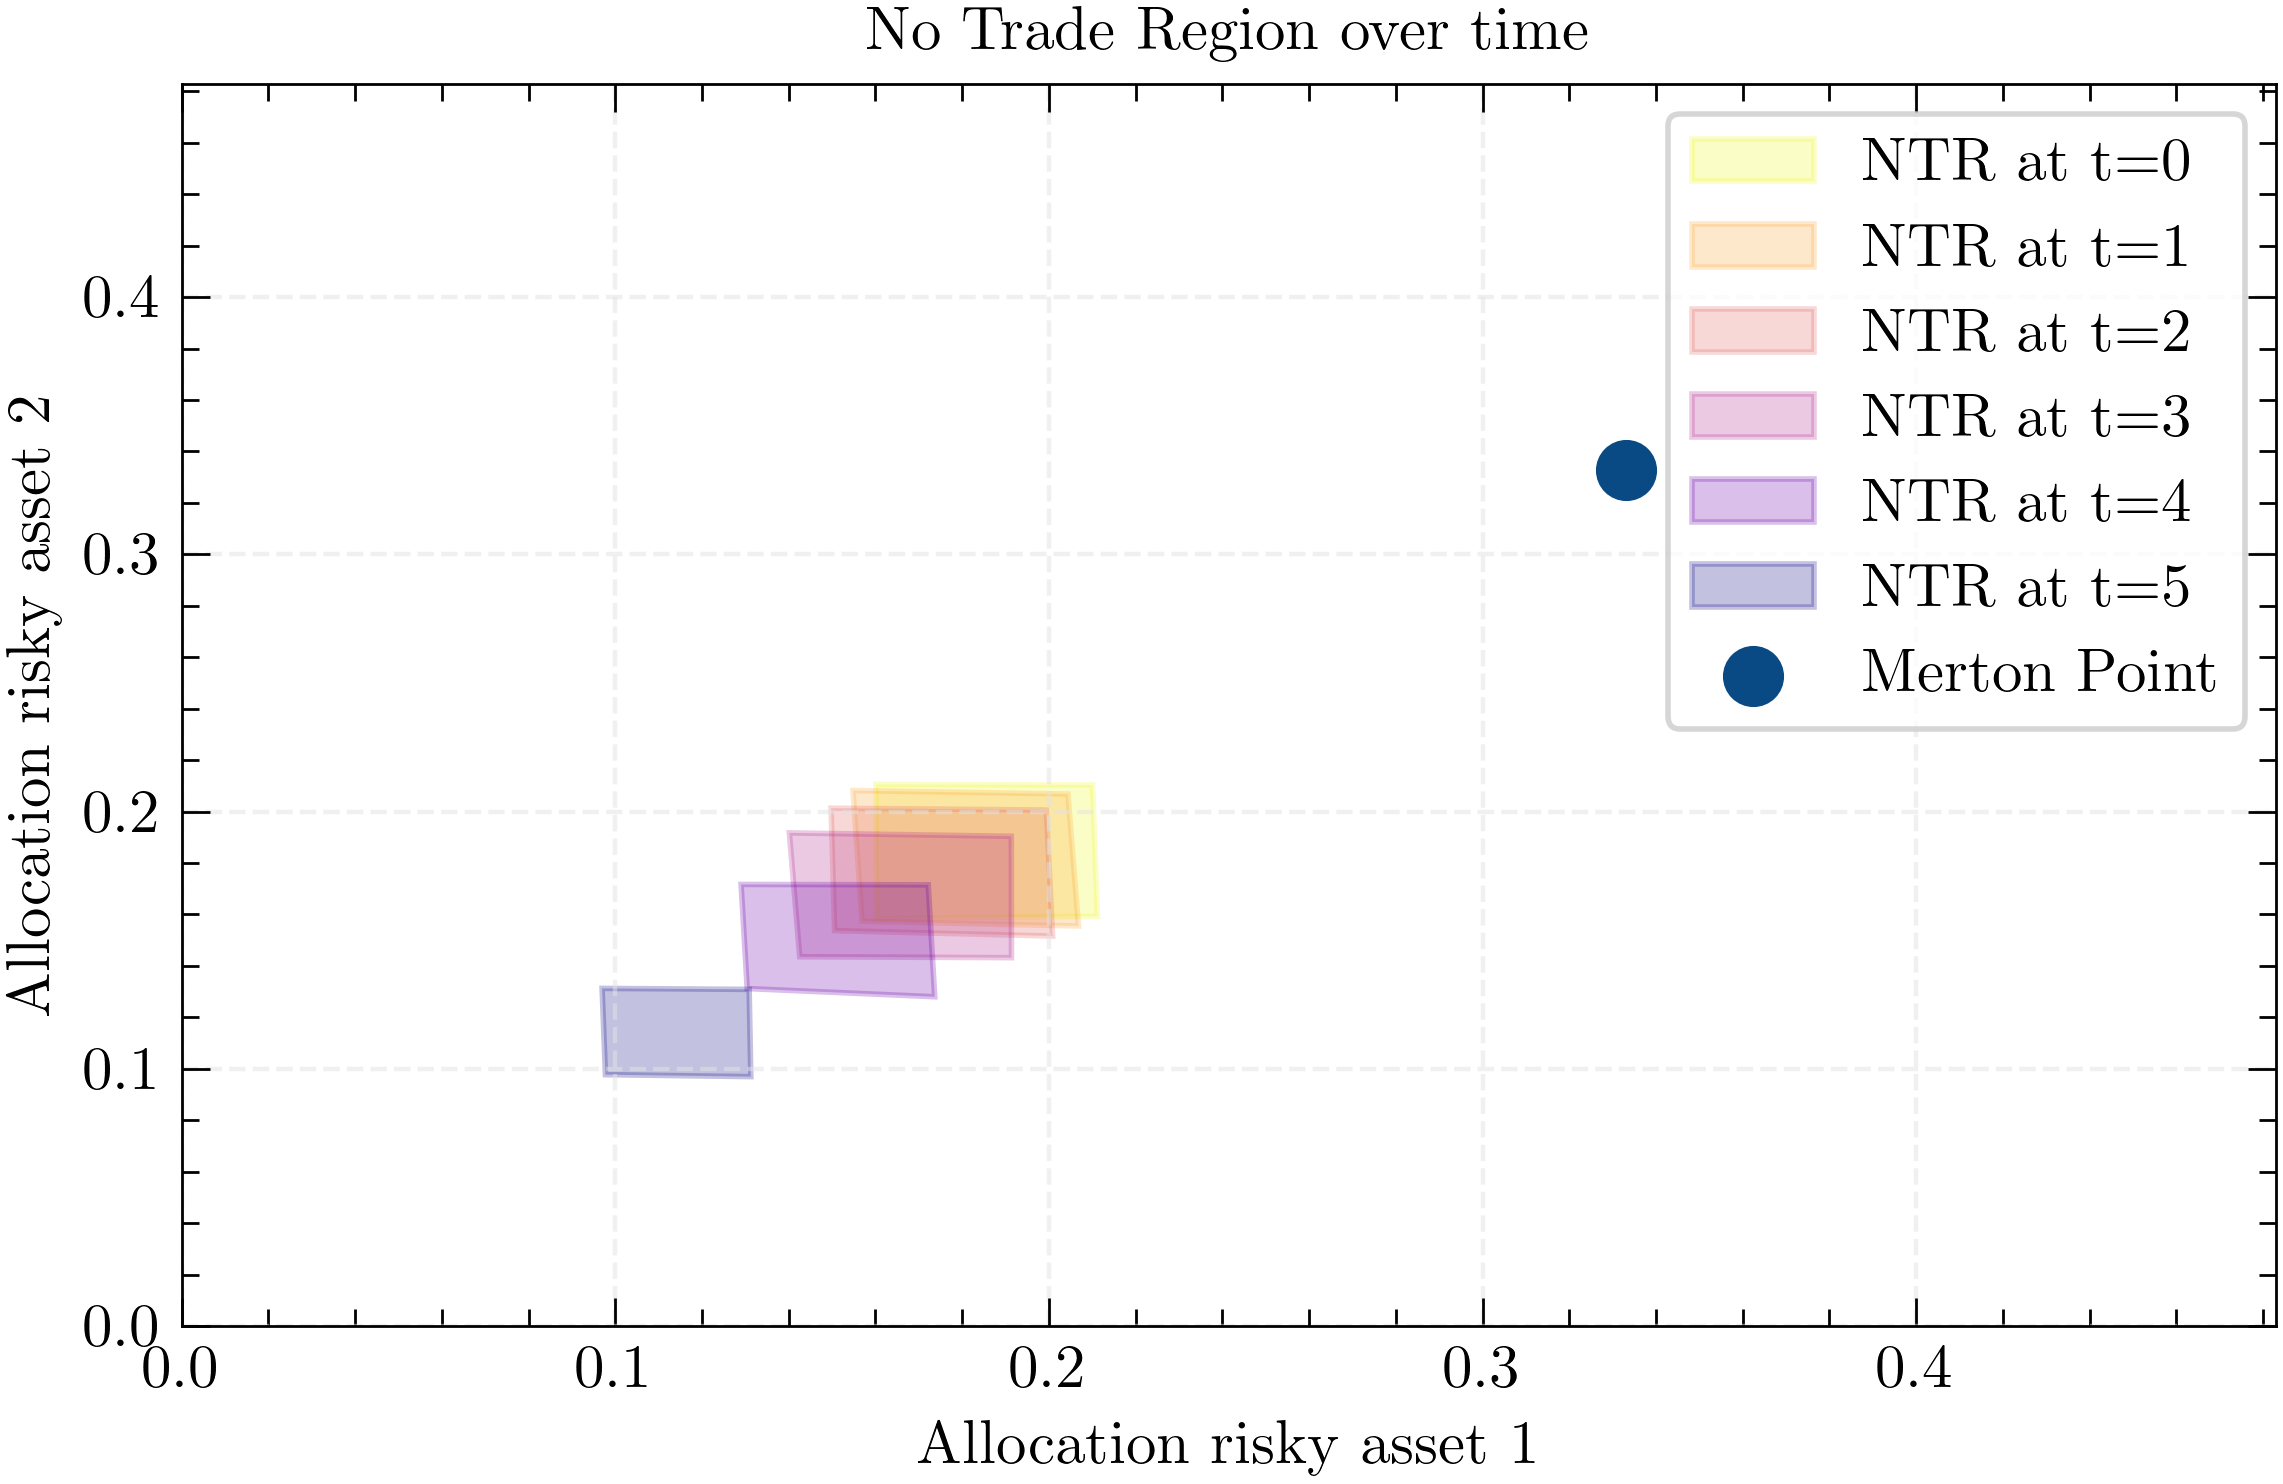
\includegraphics[scale = 0.45]{NTR_Cai_Identical_d2_tau_0.005__with_consumption_Over_Time_t_5.png}
        \caption{No Trade Region for i.i.d parameters over time with consumption.}
        \label{fig:NTR_2d_iid_with_consumption_over_time}
    \end{subfigure}%
    \hfill
    \begin{subfigure}[t]{0.48\textwidth}
        \centering
        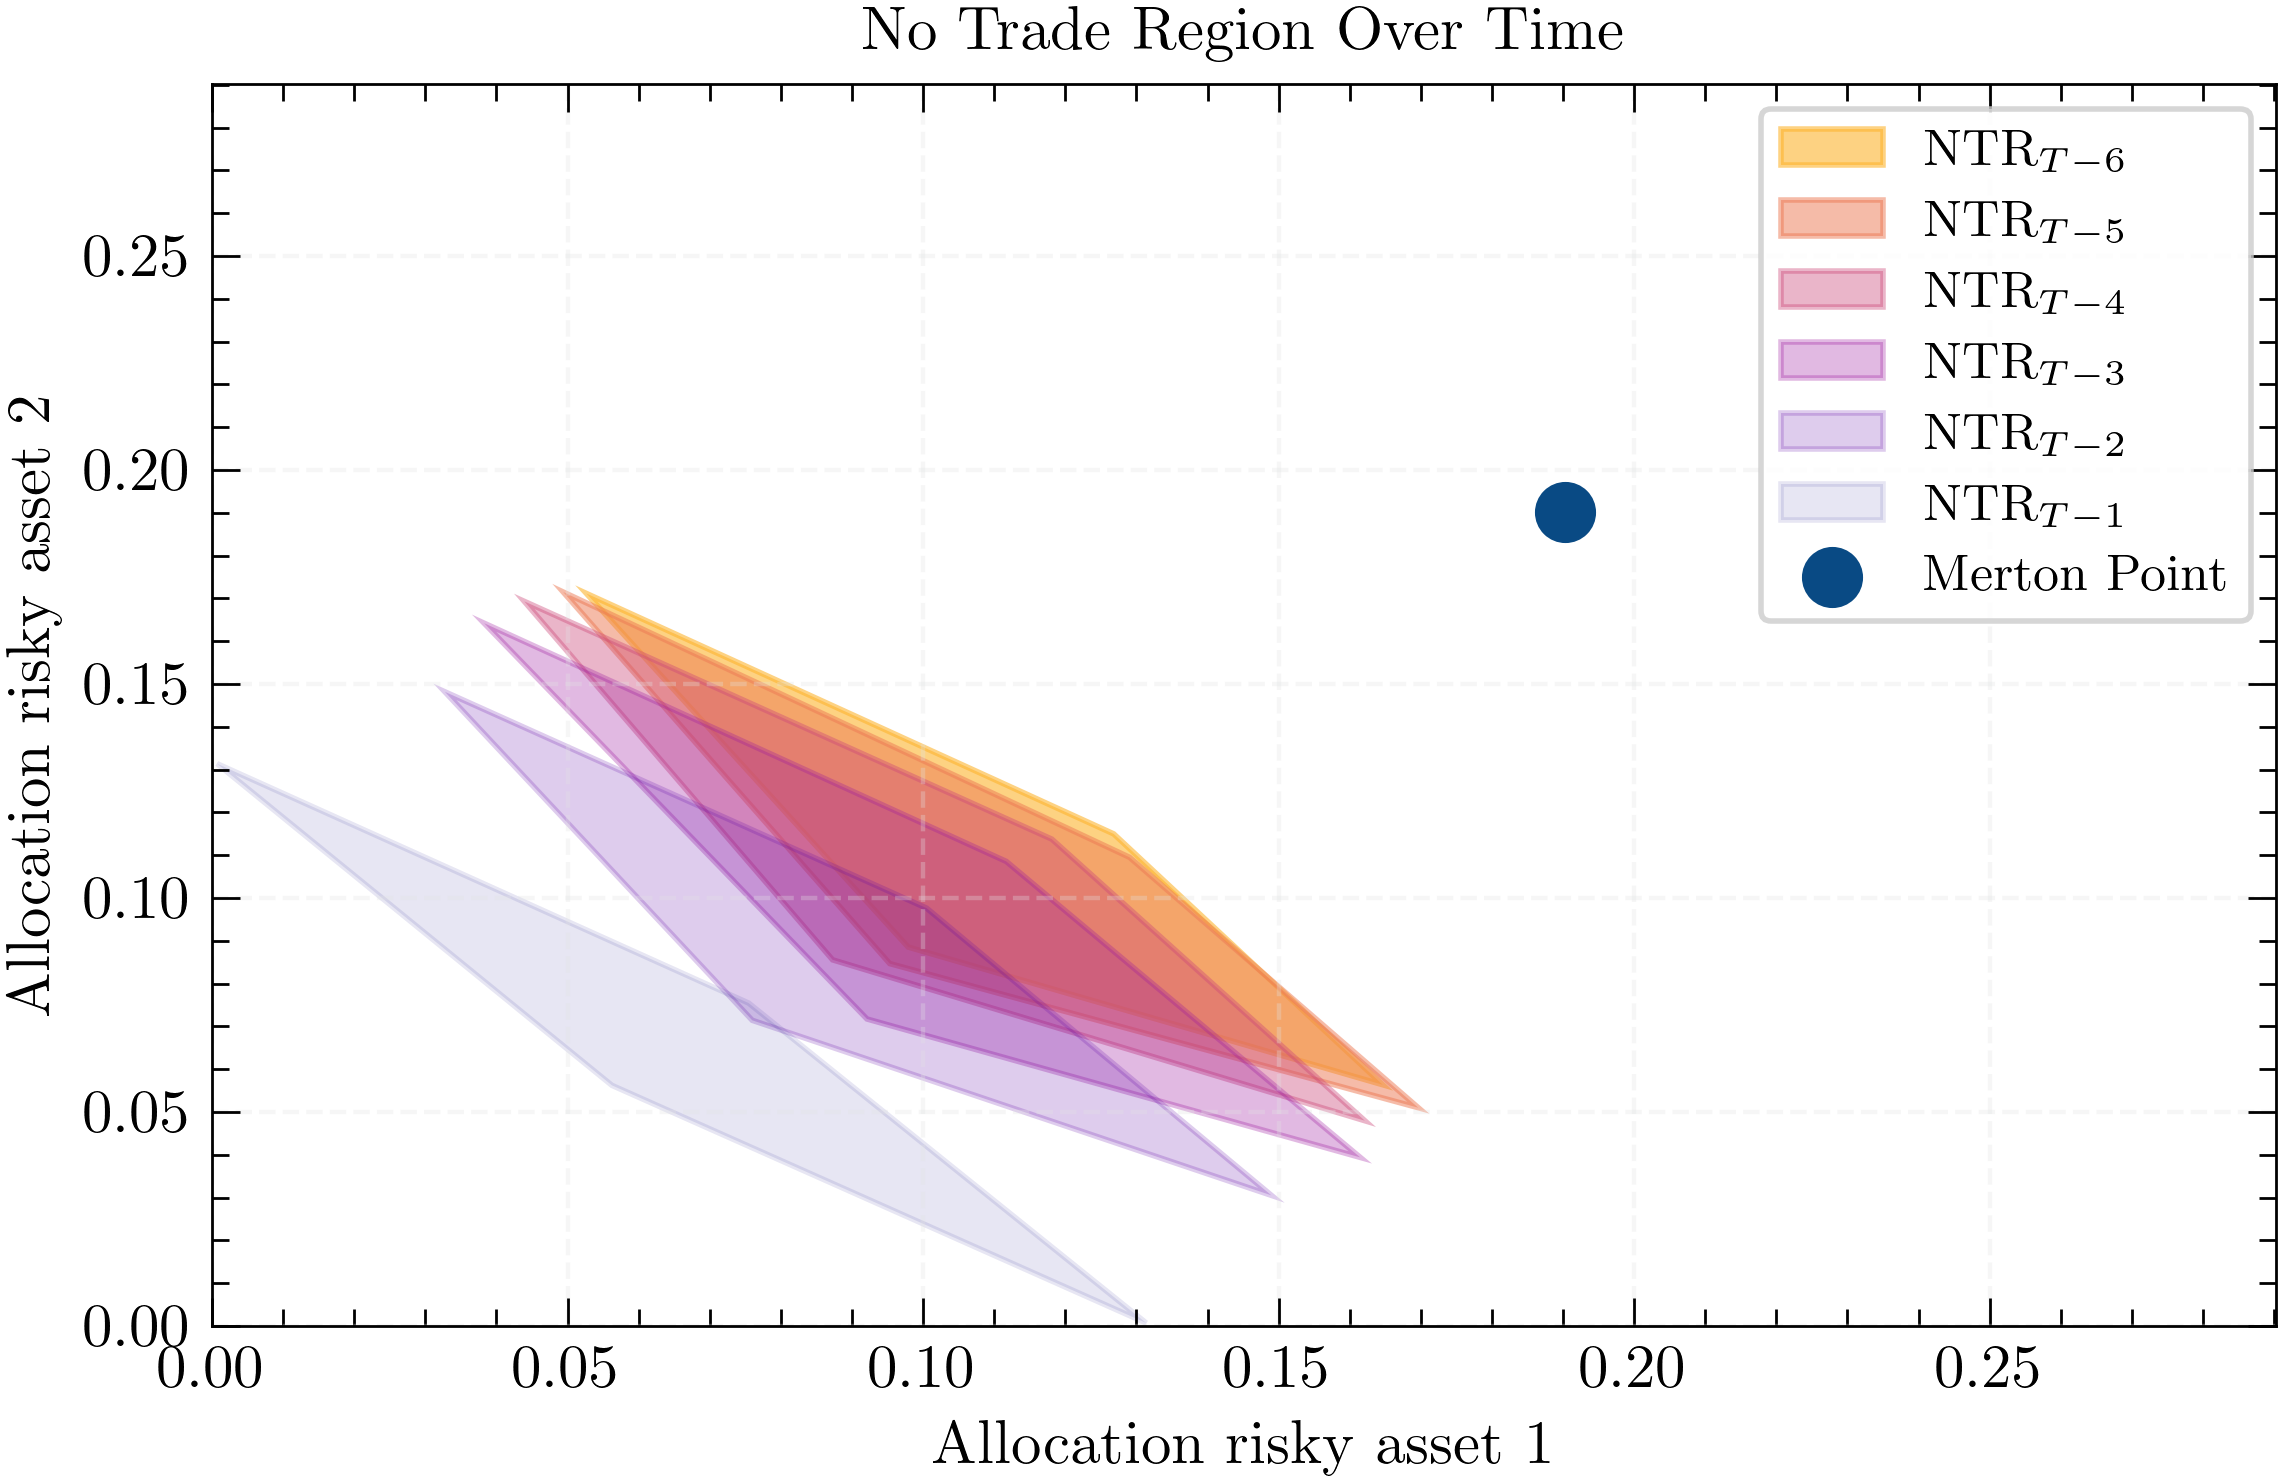
\includegraphics[scale = 0.45]{NTR_Cai_High_Correlation_d2_tau_0.005__with_consumption_Over_Time_t_5.png}
        \caption{No Trade Region for high correlation parameters over time with consumption.}
        \label{fig:NTR_2d_high_correlation_with_consumption_over_time}
    \end{subfigure}
    % Overall caption
    \caption{Comparison of No Trade Regions over time with consumption.}
    \floatfoot{The No-Trade regions are plotted over the entire investment horizon $[0, T-1]$.}
\end{figure}

Note that when consumption is included, the \ac{NTR} no longer encapulates the Merton point at any time point.
Furthermore the \ac{NTR} now moves over time, towards the origin, as opposed to the case without consumption,
where the \ac{NTR} was static for all time points except the next to last period (last period with trading decisions).

This behaviour is consistent in higher dimensions. 

\begin{figure}[!ht]
    \centering
    \begin{subfigure}[t]{0.48\textwidth}
        \centering
        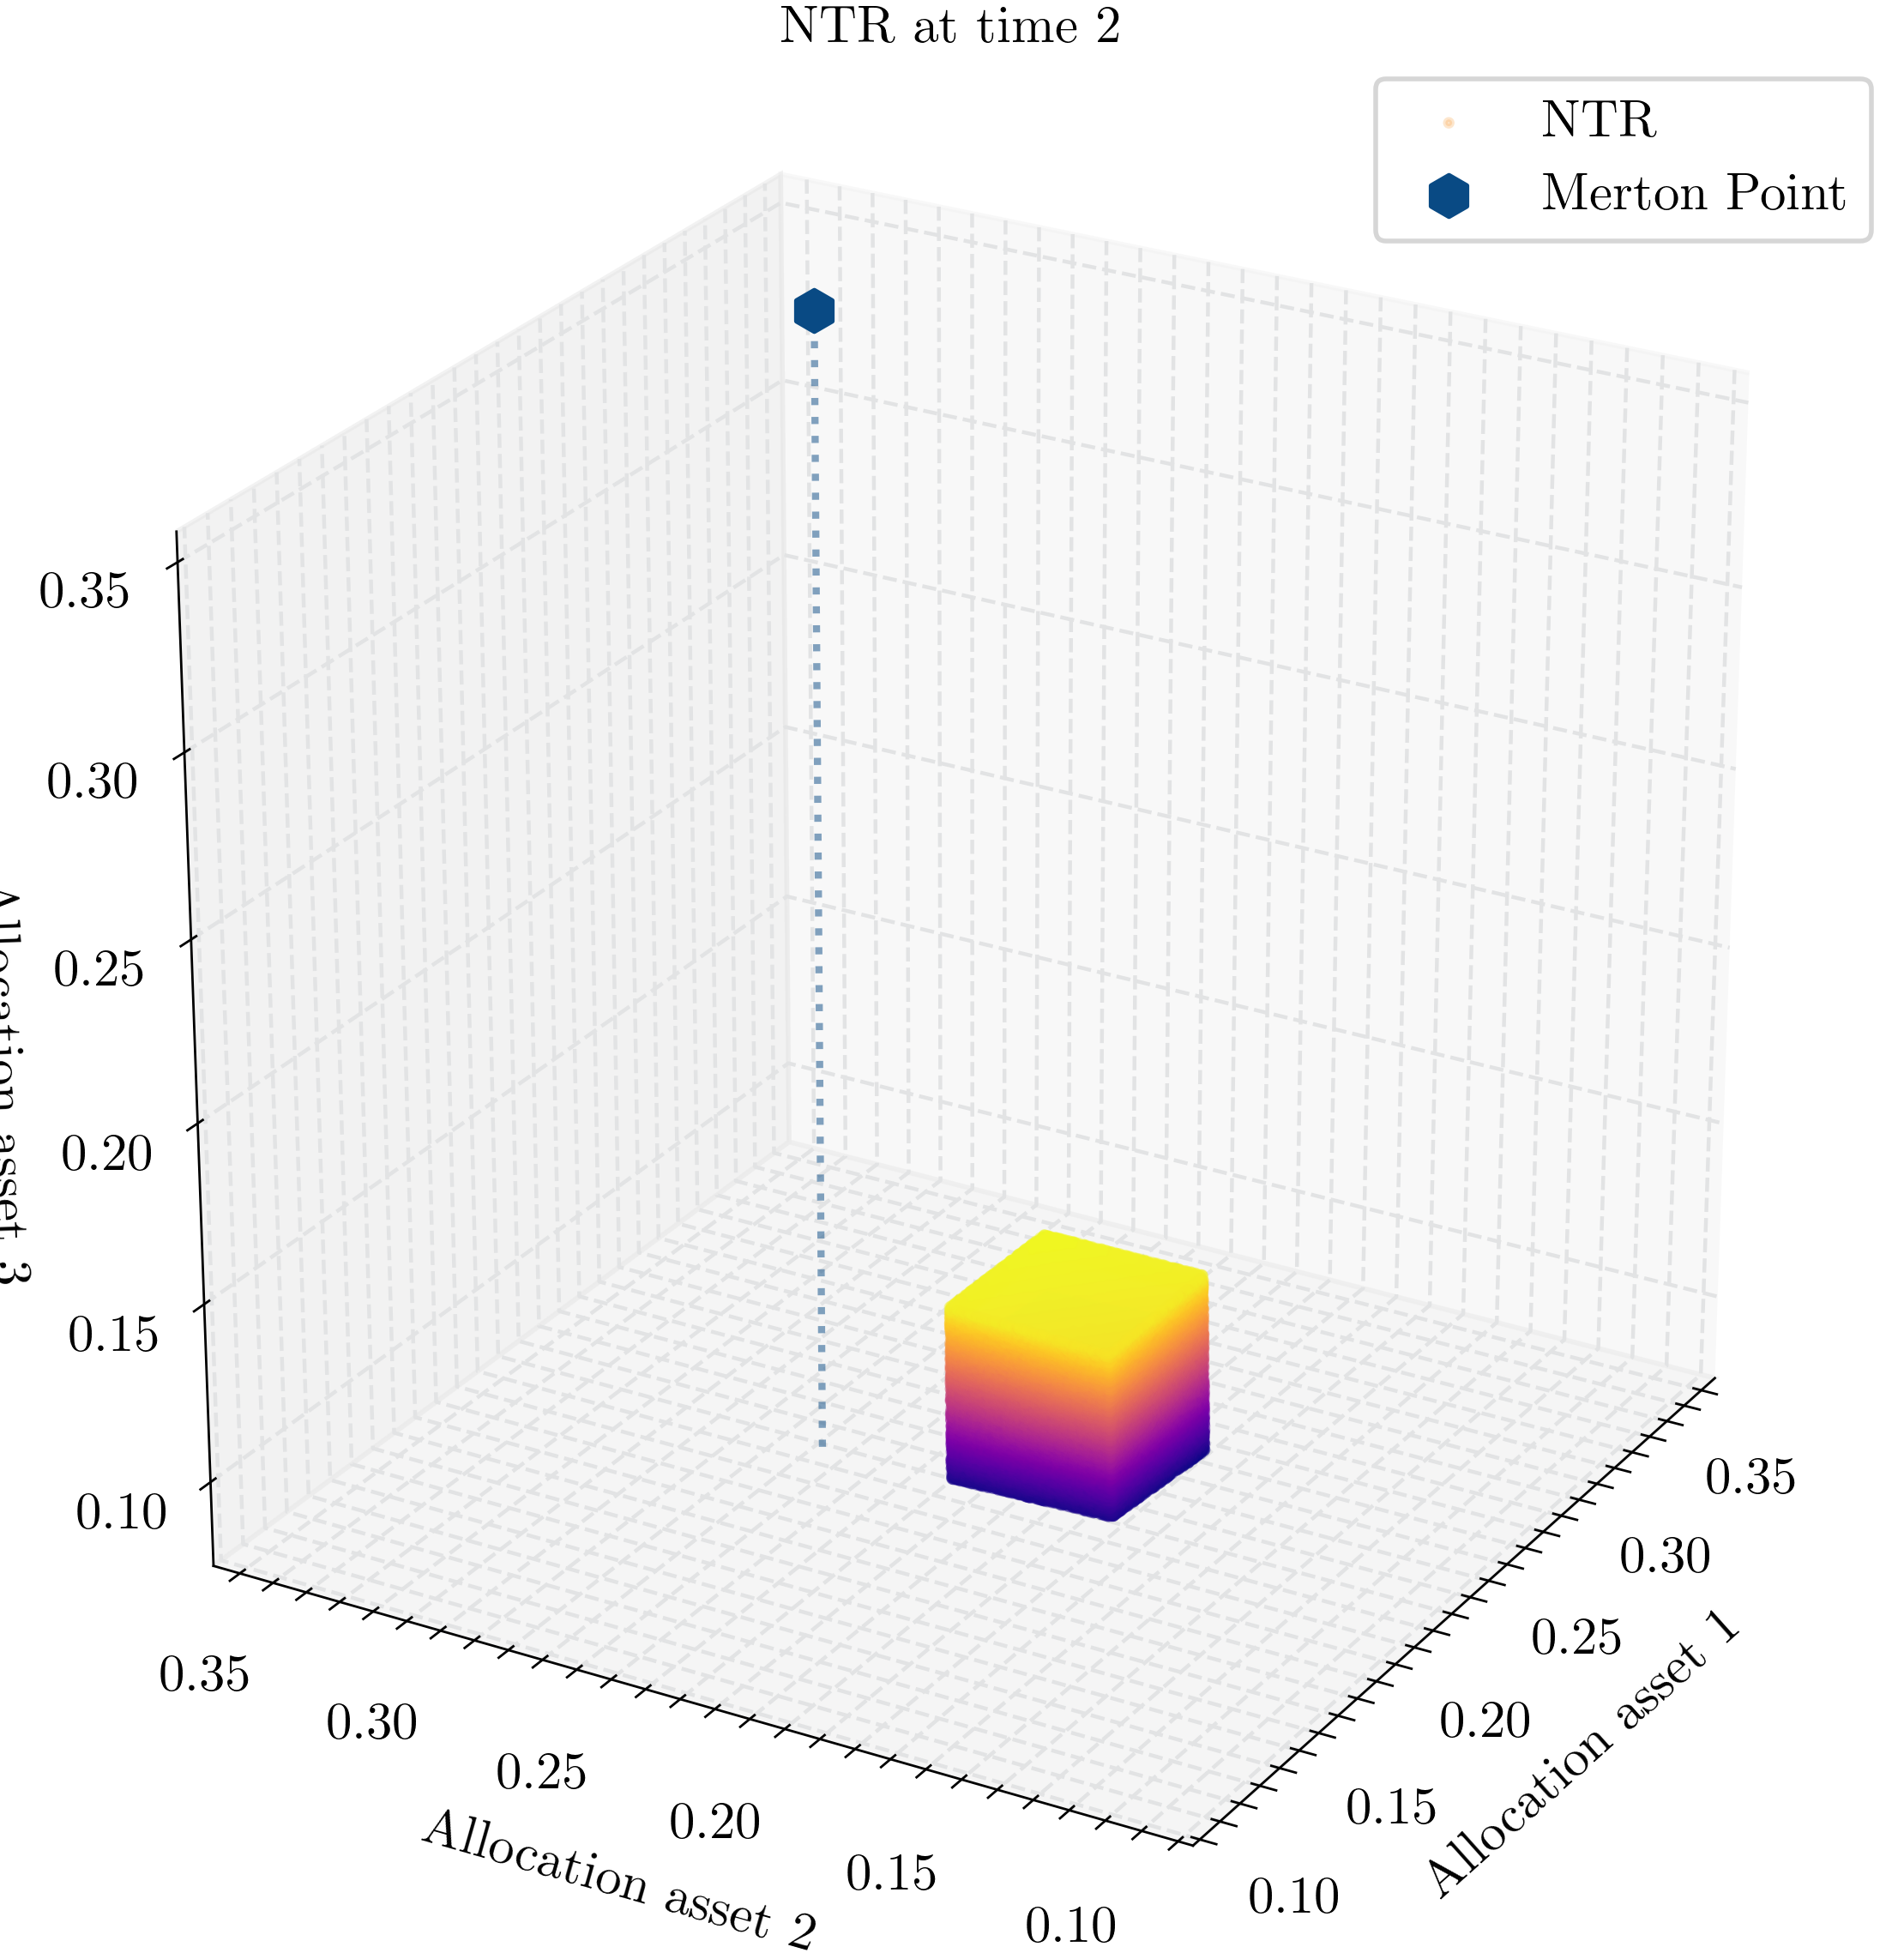
\includegraphics[scale = 0.45]{NTR_Cai_Identical_d3_tau_0.005__with_consumption_t_2.png}
        \caption{No Trade Region for i.i.d parameters with consumption in 3d.}
        % \label{fig:NTR_2d_iid_with_consumption_over_time}
    \end{subfigure}%
    \hfill
    \begin{subfigure}[t]{0.48\textwidth}
        \centering
        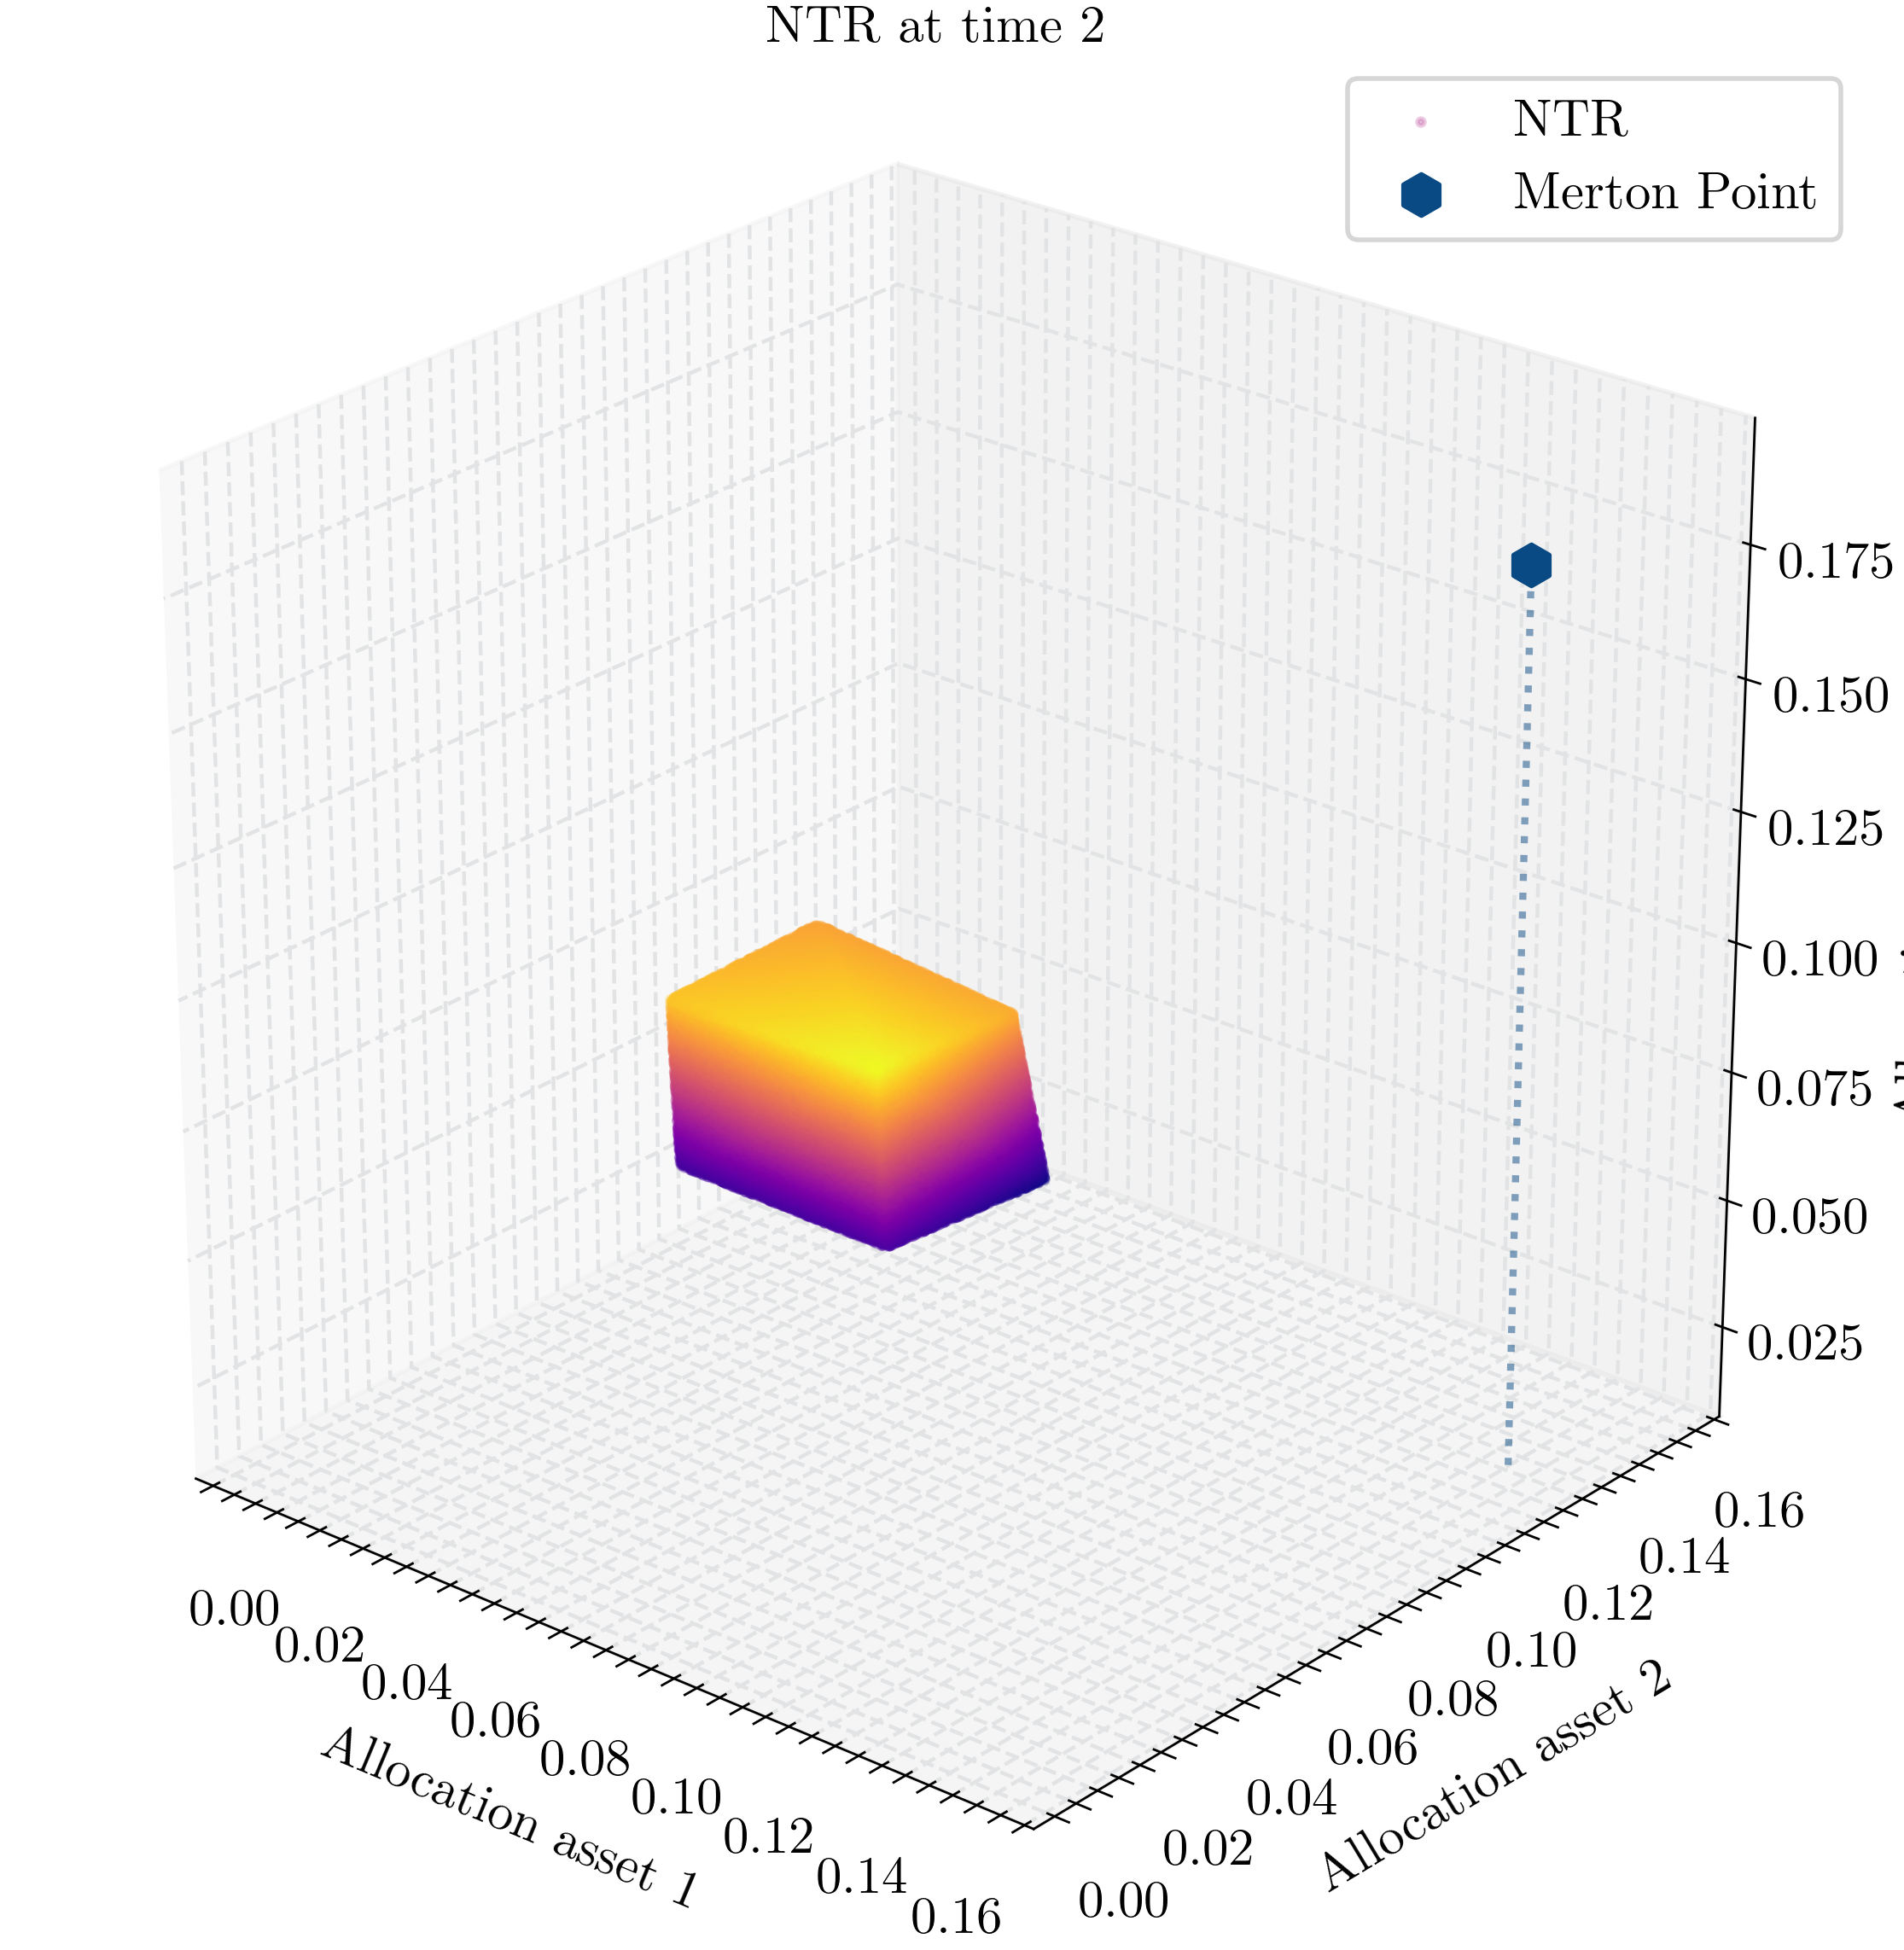
\includegraphics[scale = 0.45]{NTR_Schober_Parameters_d3_tau_0.005__with_consumption_t_2.png}
        \caption{No Trade Region for Schober parameters with consumption in 3d.}
        % \label{fig:NTR_2d_high_correlation_with_consumption_over_time}
    \end{subfigure}
    % Overall caption
    \caption{No trade regions with consumption in multiple dimensions.}
    \floatfoot{The No-Trade regions are plotted at time $t=2$.}
\end{figure}


\subsection{Dynamic Portfolio Choice with fixed costs} \label{Subsection: Results_WithConsumption}
I now consider the base model with fixed transaction costs, and no consumption.
From \autocite{Dybvig2020} i know that the \ac{NTR} is no longer rectangular when we only consider fixed costs, but instead circular with the merton point in the middle.
This poses a problem for my current sampling scheme, which leverages our predetermined knowledge of the geometric shape of the \ac{NTR}.
As i noted in Section \ref{subsubsection: Sample}, in order to effectively sample points for the \ac{NTR} approximation, i now need to 
sample points, such that when they hit the \ac{NTR} these points are evenly distributed on the sphere, in order to approximate the \ac{NTR} correctly.\\
The fixed costs pose further problems for the solution algorithm. In order to see this a little intuition is needed.

Transaction costs no longer scale, but are treated as a \textit{sunk cost}, the moment the decision to trade is made. Hence if trading is optimal, the investor will trade to the optimal point,
and if trading is sub-optimal then no trading will occur. The problem is therefore first of all a trading decision problem, and if trading is optimal, then the investor will trade to the merton point.

This is in stark contrast to the proportional case, where the trading trajectory from outside the \ac{NTR} was to the border of the \ac{NTR}, and the \ac{NTR} approximation could be done by sampling points on the border of the feasible space.

Now, any point sampled outside the \ac{NTR} trades to the merton point, and i need to construct a new strategy, in order to efficiently construct the \ac{NTR}.

Furthermore, the transaction cost function is now an indicator function, depending on a threshhold, i.e $\sum^{k}_{i=1} \delta^{+}_{i,t} + \delta^{-}_{i,t}  > 0$.
This is non-differentiable at the kink, $\sum^{k}_{i=1} \delta^{+}_{i,t} + \delta^{-}_{i,t} =0$ , which is a critical point, which i have to deal with, in order to solve the optimization problem.

I therefore split the optimization process into two parts. I evaluate the objective function (value function), conditional on no trading ($\boldsymbol{\delta}_{t} = \mathbf{0}$), and conditional on trading ($\boldsymbol{\delta}_{t} \neq \mathbf{0}$).
Since there is no consumption decision the no-trading decision is trivial, whereas i still optimize the trading decision in order to maximize expected utility. 
By splitting the optimization process, i can avoid the the non-differentiable edge case, and the derivative with regard to fixed costs i trivial for the optimizer.
I then evaluate the value function for the no-trading decision, and the trading decision, and choose the decision which maximizes the value function.

I now consider the base model with fixed transaction costs, and no consumption. I use the simple i.i.d parameterization, with $2$ assets and solve the optimization problem for the next to last period $T-1$,
over an evenly spaced grid of points. I do this in order to verify that the solution algorithm works as intended, and that the \ac{NTR} is circular as expected, conflicting with my prior assumptions for the proportional case.
I set the fixed costs to $0.005\%$ of the investors total wealth, at any time point, and solve at a very fine grid of points, in order to approximate the \ac{NTR} correctly.
I find that the \ac{NTR} is circular as expected, and the solution algorithm works as intended. I therefore proceed with generating a strategy for dealing with fixed costs, which can leverage my new found knowledge of the \ac{NTR}.
\begin{figure}[!ht]
    \centering
    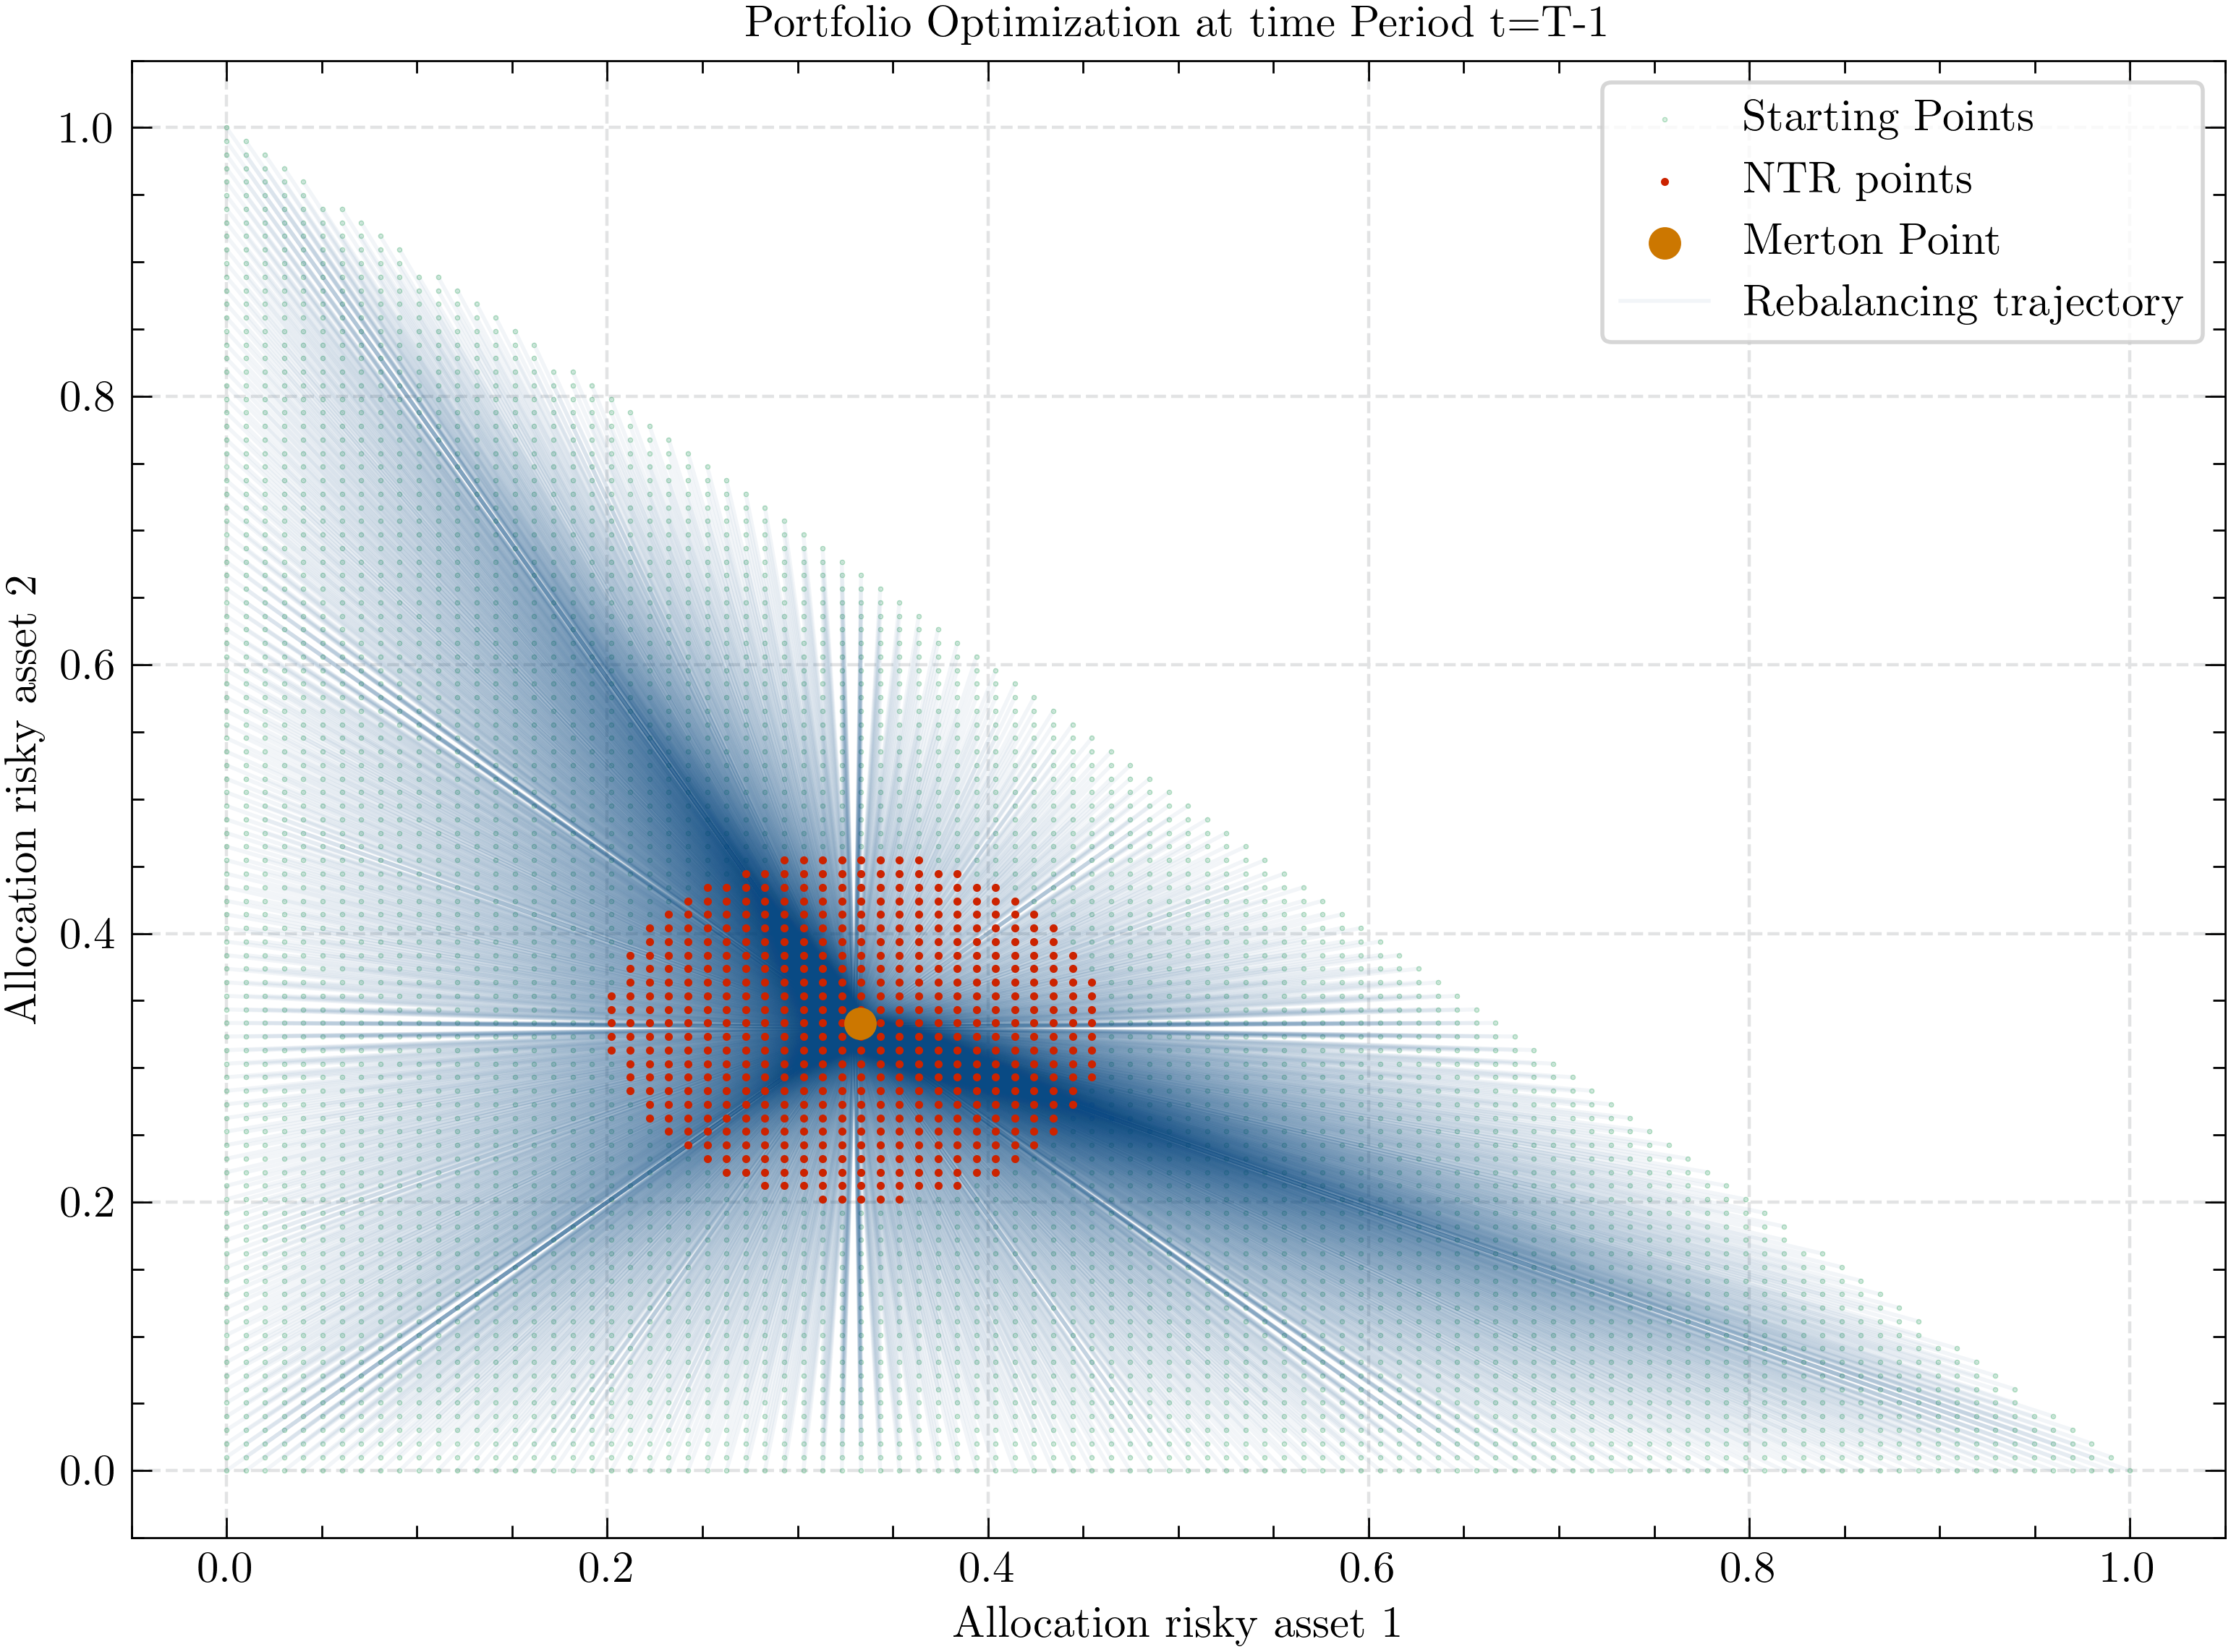
\includegraphics[scale = 0.44]{Verify_NTR_FixedCai_Identical_t_5.png}
    \caption{Solution to the i.i.d case with fixed costs, 2 assets in period $T-1$.}
    \label{fig:NTR_2d_high_correlation_with_consumption_over_time}
    \floatfoot{The optimization scheme ran with $5044$ evenly spaced grid points. The points are plotted in the feasible space, and the \ac{NTR} is the convex hull of these points.}
\end{figure}

\subsubsection{Constructing a new sampling scheme for the fixed cost NTR} \label{Subsubsection: SampleFixed}

\ifdefined\COMPILINGMAIN
% Main file is compiling this section, skip the end
\else
% \printbibliography
\end{document}
\fi